

\chapter{Turing-Welchman Bombe}

In the previous chapters, we have seen complicated manual
cryptographic techniques give rise to a set of electromechanical
tools meant to make such work tractable over short time periods.
Changes to the Enigma protocol would soon necessitate the
construction of one of the largest such electromechanical devices to
date, known as the {\bf{Bombe}}.

\subsection{Changes to the Enigma Protocol}
Recall that during the use of the Polish Bomba, operators were
instructed to send their window setting (\emph{Grundstellung}) in
plaintext, and then use this to doubly encode their message key
(\emph{Spruchschlüssel}). Starting in 1940, a small but impactful
change was made to the Enigma encryption protocol for the Army and
Air Force -- operators were instructed to send their encoded message
key only once.
\\\\The Polish Bomba relied on relationships between the doubly
encoded message key to function, without such relationships all the
previously mentioned tools became useless. World War II had begun and
the need for intelligence material was greater than ever. Thus,
British intelligence brought a group of crypt-analysts,
mathematicians, historians, linguists, and more, to Bletchley Park to
engage in a large-scale attempt to break the Enigma machine with this
new protocol.
\\\\No name is more well known from this operation than that of Alan
Turing, whose work went on to become the foundations of modern
computer science. Turing needed to find a new means of attacking the
Enigma encryption that could no longer rely on the doubly enciphered
message key. Consider that the reliance on the doubly enciphered
message key was really just a reliance on the knowledge that two
letters encoded the same plaintext at specific intervals of distance.
Thus, Turing began engineering a method of deducing daily keys via a
known plaintext attack.

% As discussed in CITE the \emph{Grundstellung} rotor
% position was sent along with the daily key and an operator chose a
% \emph{Spruchschlusse} to
% encode twice at the start of a message. Later iterations of this
% protocol removed the \emph{Grundstellung}
% from key sheets.
% \\\\These new key sheets contained the following columns
% columns \emph{Tag/Datum}, \emph{Walzenlage}, \emph{Ringstellung},
% \emph{Steckerverbindungen}, and \emph{Kenngruppen}
% \\\\Notice the removal of the \emph{Grundstellung} as well as the
% addition of the \emph{Kenngruppen}. The \emph{Kenngruppen} were a set of
% four trigrams used to identify which setting was being used to encode
% a message, this is particularly useful if trying to decode a message
% using a prior day's key.
% The operator would choose a trigram from the the \emph{Kenngruppen},
% append two letters to the front of the trigram,
% and this five letter combination (known as the
% \emph{Buchstabenkenngruppe}) would preceed the message being sent.
% If a message
% was sent in multiple segments, multiple \emph{Buchstabenkenngruppe}
% were used to start each segment.
% \\\\When sending a message the operator was to use the following protocol
% \begin{enumerate}[I.]
%   \item The time at which the message was sent is listed
%   \item The number of parts which the message contained is listed
%   \item Which message part is being sent is listed
%   \item The length of the message part (not including
%         \emph{Buchstabenkenngruppe}) is listed
%   \item A \emph{Grundstellung} rotor position is chosen and listed
%   \item A \emph{Spruchschlüssel} rotor position is chosen and encoded
%         using the \emph{Grundstellung}, this is listed
%   \item The \emph{Buchstabenkenngruppe} is listed
%   \item The message part encoded using the daily key and the
%         \emph{Spruchschlüssel} position is listed
% \end{enumerate}
% It is clear that with this protocol, the Polish Bomba could no longer
% deduce the necessary
% details to decrypt Enigma messages. All of the permutation
% information contained in the original key distribution
% protocol was removed and a new method needed to be derived for
% infering information about the daily key.
% \section{Loops}
% The removal of the double encoded \emph{Spruchschlüssel} does not
% mean that permutation information cannot be stored elsewhere in the message.
% For the sake of argument, let us say we knew that our encrypted
% message had plaintext encoding

% \begin{center}
% \begin{tikzpicture}[node distance=1cm, every node/.style={draw,
% circle, minimum height=0.1cm, minimum width=0.1cm}]

%     % Centering the diagram
%     \node (a1) [] {D};
%     \node (a2) [right=0.1cm of a1] {Y};
%     \node (a3) [right=0.1cm of a2] {Y};
%     \node (a4) [right=0.1cm of a3] {Y};
%     \node (a5) [right=0.1cm of a4] {Y};
%     \node (a6) [right=0.1cm of a5] {Y};
%     \node (a7) [right=0.1cm of a6] {X };
%     \node (a8) [right=0.1cm of a7] {Y};
%     \node (a9) [right=0.1cm of a8] {Y};
%     \node (a10) [right=0.1cm of a9] {Y};
%     \node (a11) [right=0.1cm of a10] {X};

%     % Nodes for ciphertext
%     \node (x1) [below=1cm of a1] {A};
%     \node (x2) [below=1cm of a2] {B};
%     \node (x3) [below=1cm of a3] {R};
%     \node (x4) [below=1cm of a4] {A};
%     \node (x5) [below=1cm of a5] {C};
%     \node (x6) [below=1cm of a6] {A};
%     \node (x7) [below=1cm of a7] {D};
%     \node (x8) [below=1cm of a8] {A};
%     \node (x9) [below=1cm of a9] {B};
%     \node (x10) [below=1cm of a10] {R};
%     \node (x11) [below=1cm of a11] {A};

%     % Arrows for mapping
%     \draw[->] (a1) -- (x1) node[midway, left, draw=none, fill=none] {1};
%     \draw[->] (a2) -- (x2) node[midway, left, draw=none, fill=none] {2};
%     \draw[->] (a3) -- (x3) node[midway, left, draw=none, fill=none] {3};
%     \draw[->] (a4) -- (x4) node[midway, left, draw=none, fill=none] {4};
%     \draw[->] (a5) -- (x5) node[midway, left, draw=none, fill=none] {5};
%     \draw[->] (a6) -- (x6) node[midway, left, draw=none, fill=none] {6};
%     \draw[->] (a7) -- (x7) node[midway, left, draw=none, fill=none] {7};
%     \draw[->] (a8) -- (x8) node[midway, left, draw=none, fill=none] {8};
%     \draw[->] (a9) -- (x9) node[midway, left, draw=none, fill=none] {9};
%     \draw[->] (a10) -- (x10) node[midway, left, draw=none, fill=none] {10};
%     \draw[->] (a11) -- (x11) node[midway, left, draw=none, fill=none] {11};

%     \end{tikzpicture}
% \end{center}

% Where the top row is the ciphertext and the bottom is the
% plaintext, further, the number in each mapping indicates how many
% steps away we are from the rotor
% positions when we began encoding the message.

% \begin{center}
%     \begin{tikzpicture}[node distance=1cm, every node/.style={draw,
% circle, minimum height=0.1cm, minimum width=0.1cm}]
%         \node (A) at (90:1.5) {$A$};
%         \node (D) at (210:1.5) {$D$};
%         \node (X) at (330:1.5) {$X$};

%         \draw[->, bend right=45] (A) to node[midway, draw=none,
% above] {1} (D);
%         \draw[->, bend right=45] (D) to node[midway, draw=none,
% above] {7} (X);
%         \draw[->, bend right=45] (X) to node[midway, draw=none,
% above] {11} (A);
%       \end{tikzpicture}
% \end{center}

% Recall
% \begin{align*}
%     E_1 &=
% P^{-1}\theta_1R_1^{-1}\theta_1^{-1}R_2^{-1}R_3^{-1}MR_3R_2\theta_1^{-1}R_1\theta_1P
%     \\E_7 &=
% P^{-1}\theta_7R_1^{-1}\theta_7^{-1}R_2^{-1}R_3^{-1}MR_3R_2\theta_7^{-1}R_1\theta_7P
%     \\E_{11} &=
% P^{-1}\theta_{11}R_1^{-1}\theta_{11}^{-1}R_2^{-1}R_3^{-1}MR_3R_2\theta_{11}^{-1}R_1\theta_{11}P
% \end{align*}
% Then it follows that our loop can be represented by
% \begin{align*}
%     \sigma &= E_{11}\circ E_7 \circ E_{1}
% \end{align*}
% and we see that all the intermediate plugboard settings cancel out.
% Lets isolate the plugboard settings by letting
% $\overline{\sigma}$ represent $\sigma$ without the use of the
% plugboard for input and output, then
% \[
%     \sigma = P^{-1}\overline{\sigma}P
% \]
% We have that
% \begin{align*}
%     \sigma(A) &= A
%     \\\iff (P^{-1}\overline{\sigma}P)(A) &= A
%     \\\iff \overline{\sigma}(P(A)) &= P(A)
% \end{align*}

% Suppose that our initial rotor position was correct, then certainly
% our $\overline{\sigma}$ is correct. We can make a hypothesis
% that $A$ is steckered to $K$ in the plugboard. Suppose we find that
% $\overline{\sigma}(K) \ne K$, then $\sigma(A)\ne A$ and our loop is
% broken, breaking our assumptions, thus $A$ must not be steckered to $K$.
% But this will actually elimiate more hypotheses than just $A$ being
% steckered to $K$. We know that $\overline{\sigma}(K)$ is some
% letter which is not $K$. So we continue with a new hypothesis that
% $A$ is steckered to
% $\overline{\sigma}(K)$ and if we find
% $\overline{\sigma}(\overline{\sigma}(K)) \ne \overline{\sigma}(K)$,
% then we have further eliminated this possibility.
% Each new hypothesis suggests that $A$ is steckered to
% $\overline{\sigma}^{i}(K)$ which will be shown to be false if
% $\overline{\sigma}^{i+1}(K) \ne \overline{\sigma}^{i}(K)$. What if
% we find that
% $\overline{\sigma}^{i+1}(K) = \overline{\sigma}^i(K)$ at some
% point? This cannot happen since
% \begin{center}
%         \begin{align*}
%             &\overline{\sigma}^{i+1}(K) = \overline{\sigma}^i(K)
%             \\\Rightarrow \text{
% }&\overline{\sigma}^{-i}\circ\overline{\sigma}^{i+1}(K) =
% \overline\sigma^{-i}\circ\overline{\sigma}^i(K)
%             \\\Rightarrow \text{ }&\overline{\sigma}(K) = K
%         \end{align*}
% \end{center}
% which by supposition is false. Then we can continue in our
% hypotheses until we eventually reach a cycle where $\overline\sigma^i(K) = K$.
% Then we gather a set of impossible steckerings, that is
% \begin{align*}
%     P(A) \notin \{\text{ }\overline{\sigma}^i(K)\text{ }\vert\text{
% }i\in\mathbb{N}\}
% \end{align*}
% \\\\The notation we are using can be simplified significantly. The
% set $\{\text{ }\overline{\sigma}^i(K)\text{ }\vert\text{
% }i\in\mathbb{N}\}$ is equivalent to the orbit of $K$ via the group
% action of the
% cyclic subgroup $\langle\overline{\sigma}\rangle$ which can be
% denoted $\langle\overline{\sigma}\rangle\cdot K$.
% \\\\We then have several cases
% \begin{enumerate}
%     \item If $|\langle\overline{\sigma}\rangle\cdot K| = 26$, then
% $A$ cannot be steckered to anything which is clearly
%     impossible, thus our rotor position must be incorrect.
%     \item If $|\langle\overline{\sigma}\rangle\cdot K| = 25$, then
% $A$ can only be steckered to the remaining letter \\$\{A,\dots,Z\} -
%     \langle \overline{\sigma} \rangle\cdot K$
%     \item If $|\langle\overline{\sigma}\rangle\cdot K| = 1$, in
% this case we must have intially had $\overline{\sigma}(K) = K$ so we have not
%     eliminated any possibilities.
% \end{enumerate}

% https://archive.org/details/enigmabattleforc0000seba/page/82/mode/2up?q=herivel
% %
\subsection{Herivel Tip}
While Turing was developing his plaintext attack that ultimately
culminated in the creation of the Bombe, there was a period of time
that some have called a "blackout" in which little to no Enigma
messages could be deciphered. During this time, Bletchley Park
cryptanalyst John Herivel had a simple idea. When operators set their
ring settings as described by the key sheet they would place their
wheels in the machine in the order described, and they would then
turn the outer ring on each wheel so that the corresponding ring
setting letter was at the top of the wheel. If the operator was
particularly lazy, this was \emph{all} they did, or if they were only
slightly lazy, they may turn the wheels a couple turns forward or
back. Regardless, this meant that many operators began enciphering
their messages with a window setting that was nearly identical to the
ring setting. Thus, by looking at several operators first messages of
the day, we would see several cluster around a particular setting
that is likely to be the ring setting. Such an insight became known
as the {\bf{Herevil tip}}.
\\\\With the Herevil tip, we could determine a likely ring setting.
Then by either brute force or use of the clock method, we could
determine the rotor order. Then finally, as we did to recover the
plugboard from the Bomba in section~\ref{bomba_plugboard}, we could
even recover the plugboard settings. Thus, purely by virtue of
operator error, we could recover the entire daily key.
\\\\Ultimatley this only helped them to decipher messages within a
particular network of operators known as the "Red network". However,
as we will later see, access to a set of plaintext from messages will
become a vital component of our plaintext attack.
\section{Plaintext Attack}

Suppose we knew the plaintext which had been enciphered into a
particular Enigma transmission.
Consider the following mapping,
\begin{center}
	\begin{tikzpicture}[node distance=1cm, every node/.style={draw,
					circle, minimum height=0.1cm, minimum width=0.1cm}]

		% Centering the diagram
		\node (a1) [] {\texttt{D}};
		\node (a2) [right=0.1cm of a1] {\texttt{Y}};
		\node (a3) [right=0.1cm of a2] {\texttt{Y}};
		\node (a4) [right=0.1cm of a3] {\texttt{Y}};
		\node (a5) [right=0.1cm of a4] {\texttt{Y}};
		\node (a6) [right=0.1cm of a5] {\texttt{Y}};
		\node (a7) [right=0.1cm of a6] {\texttt{X }};
		\node (a8) [right=0.1cm of a7] {\texttt{Y}};
		\node (a9) [right=0.1cm of a8] {\texttt{Y}};
		\node (a10) [right=0.1cm of a9] {\texttt{Y}};
		\node (a11) [right=0.1cm of a10] {\texttt{X}};

		% Nodes for ciphertext
		\node (x1) [below=1cm of a1] {\texttt{A}};
		\node (x2) [below=1cm of a2] {\texttt{B}};
		\node (x3) [below=1cm of a3] {\texttt{R}};
		\node (x4) [below=1cm of a4] {\texttt{A}};
		\node (x5) [below=1cm of a5] {\texttt{C}};
		\node (x6) [below=1cm of a6] {\texttt{A}};
		\node (x7) [below=1cm of a7] {\texttt{D}};
		\node (x8) [below=1cm of a8] {\texttt{A}};
		\node (x9) [below=1cm of a9] {\texttt{B}};
		\node (x10) [below=1cm of a10] {\texttt{R}};
		\node (x11) [below=1cm of a11] {\texttt{A}};

		% Arrows for mapping
		\draw[->] (a1) -- (x1) node[midway, left, draw=none, fill=none] {1};
		\draw[->] (a2) -- (x2) node[midway, left, draw=none, fill=none] {2};
		\draw[->] (a3) -- (x3) node[midway, left, draw=none, fill=none] {3};
		\draw[->] (a4) -- (x4) node[midway, left, draw=none, fill=none] {4};
		\draw[->] (a5) -- (x5) node[midway, left, draw=none, fill=none] {5};
		\draw[->] (a6) -- (x6) node[midway, left, draw=none, fill=none] {6};
		\draw[->] (a7) -- (x7) node[midway, left, draw=none, fill=none] {7};
		\draw[->] (a8) -- (x8) node[midway, left, draw=none, fill=none] {8};
		\draw[->] (a9) -- (x9) node[midway, left, draw=none, fill=none] {9};
		\draw[->] (a10) -- (x10) node[midway, left, draw=none, fill=none] {10};
		\draw[->] (a11) -- (x11) node[midway, left, draw=none, fill=none] {11};

	\end{tikzpicture}
\end{center}
where the top row indicates our enciphered message, the bottom row
indicates the plain-text,
and the indices on the arrows indicate how many steps forward our
Enigma machine has moved while enciphering this message.
\\\\From this pairing we have that
\begin{center}
	$\sigma_1(\texttt{A}) = {\texttt{D}}$\\
	$\sigma_7(\texttt{D}) = {\texttt{X}}$\\
	$\sigma_{11}(\texttt{X}) = {\texttt{A}}$\\
\end{center}
% Our goal is to determine which Enigma settings were used to encipher
% the message.  In order to achieve this,
% we will examine which settings maintain the relationships between the
% enciphered and plaintext letters.
% \\\\For example, any setting which maintains the above pairing must
% encipher $\texttt{A}$ to $\texttt{D}$ from the first position of
% the machine, then at
% the seventh position, it must encipher $\texttt{D}$ to
% $\texttt{X}$, and at the
% eleventh position $\texttt{X}$ must be enciphered back to
% $\texttt{A}$. It follows that if we had
% three Enigma machines connected in series, with an offset of 1, 7,
% and 11, from our initial position, then inputting $\texttt{A}$ on the first
% machine would result in an ouput of $\texttt{A}$ on the
% third machine.
Thus, $\sigma_1$, $\sigma_7$, and $\sigma_{11}$ form a loop starting
at \texttt{A}. We visualize this loop as follows
\begin{center}
	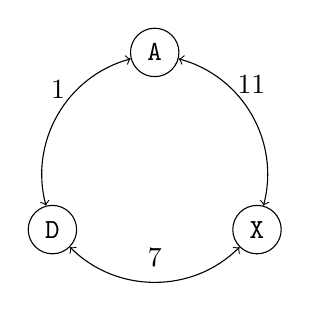
\begin{tikzpicture}[node distance=1cm, every node/.style={draw,
					circle, minimum height=0.1cm, minimum width=0.1cm}]
		\node (A) at (90:1.5) {$\texttt{A}$};
		\node (D) at (210:1.5) {$\texttt{D}$};
		\node (X) at (330:1.5) {$\texttt{X}$};

		\draw[<->, bend right=45] (A) to node[midway, draw=none, above] {1} (D);
		\draw[<->, bend right=45] (D) to node[midway, draw=none, above] {7} (X);
		\draw[<->, bend right=45] (X) to node[midway, draw=none, above] {11} (A);
	\end{tikzpicture}
\end{center}
Recall that, ignoring turnover, each $\sigma_i$ is of the form
\begin{center}
	$\sigma_i = S^{-1}P^{-(x+i)}N^{-1}P^{x+i}M^{-1}L^{-1}RLMP^{-(x+i)}NP^{x+i}S$
\end{center}
We will denote $\sigma_i$ separated from its plugboard as
\begin{center}
	$\overline{\sigma_i} =
		P^{-(x+i)}N^{-1}P^{x+i}M^{-1}L^{-1}RLMP^{-(x+i)}NP^{x+i}$
\end{center}
\noindent that is $\sigma_i = S^{-1}\overline{\sigma_i}S$
(conversely, $\overline\sigma_i = S^{-1}\sigma_iS$)\footnote{It
	should be noted that $S$ = $S^{-1}$ since the plugboard is always an
	involution}.
Then our loop is expressed by the fact that
$\sigma_{11}\sigma_7\sigma_1$ has a fixed point at $\texttt{A}$.
We also note that the intermediate plugboard settings cancel out, that is
\begin{center}
	\begin{align*}
		\sigma_{1}\sigma_7\sigma_{11} & =
		S^{-1}\overline{\sigma_{1}}SS^{-1}\overline{\sigma_7}SS^{-1}\overline{\sigma_{11}}S
		\\&= S^{-1}
		\overline{\sigma_{1}}\overline{\sigma_7}\overline{\sigma_{11}}
		S
	\end{align*}
\end{center}
We will condense this notation by defining
\begin{center}
	$\pi \coloneq \sigma_{1}\sigma_7\sigma_{11}$
\end{center}
and
\begin{center}
	$\overline{\pi} \coloneq
		\overline{\sigma_{1}}\overline{\sigma_7}\overline{\sigma_{11}}$
\end{center}
And thus we have shown $\pi = S^{-1}\overline{\pi}S$ (conversely,
$\overline\pi = S^{-1}\pi S$).
\\\\Let us hypothesize that $\texttt{A}$ is steckered in the plugboard to
$\alpha$ -- that is, $S(\texttt{A}) = \alpha$ (conversely, $S(\alpha)
	= \texttt{A}$).
It then follows that for a fixed $i\in\mathbb{N}$
\begin{center}
	\begin{align*}
		\overline{\pi}^i(\alpha) & = S\pi^i S(\alpha)
		\\&= S \pi^i(\texttt{A})
		\\&= S(\texttt{A})
	\end{align*}
\end{center}
and so we derive
\begin{center}
	$S(\texttt{A}) = \alpha \Rightarrow S(\texttt{A}) =
		\overline{\pi}^i(\alpha)\text{
		}\forall\text{ }i\in\mathbb{N}$
\end{center}
Then we have that $\texttt{A}$ must be steckered to all values in the set
$\{\overline{\pi}^i(\alpha)\text{ }\vert\text{ }i\in\mathbb{N}\}$.
We note that this set is that orbit of the element $\alpha$ under the
group action of the subgroup $\langle\overline{\pi}\rangle$ -- that is,
$\langle\overline{\pi}\rangle\cdot\alpha$.
\\\\By construction of the Enigma machine, $\texttt{A}$ cannot be steckered to
more than one value at a time, so if
$|\langle\overline{\pi}\rangle\cdot\alpha| > 1$ our initial
hypotheses that $S(\texttt{A}) = \alpha$ must have been incorrect. Further,
the above argument also illustrates that $\texttt{A}$ cannot be steckered to
any element in the orbit of $\alpha$ since
we would similarly find that the orbit of \emph{that} element was not a
singleton. Then we now have
\begin{center}
	$|\langle\overline{\pi}\rangle\cdot\alpha| > 1 \Rightarrow
		\texttt{A} \text{ cannot be steckered to any element in
		}\langle\overline{\pi}\rangle\cdot\alpha$
\end{center}
thus eliminating several elements that $\texttt{A}$ could be steckered to.
\\\\By representing $\overline\pi$ in its cycle notation we can
quickly see whether certain hypotheses are possible. For example,
suppose we found that
\begin{center}
	$\overline\pi =
		(\texttt{ABCDEF})(\texttt{GHIJK})(\texttt{L})(\texttt{MNOPQRSTUVWXYZ})$
\end{center}
If we suppose that $\texttt{A}$ is steckered to any element in the cycle
$(ABCDEF)$ we find that this
element has an orbit of length $6$ in $\langle\overline\pi\rangle$
and thus $\texttt{A}$ cannot be steckered
to any element in this cycle. Then it is clear that $\texttt{A}$ can only be
steckered to $\texttt{L}$ in this case.

\subsection{Scanning Methods}
Turing describes various methods of mechanizing the above analysis of
cycle-type to determine when we can eliminate rotor positions.
\begin{enumerate}
	\item If we examine a particular hypothesis, say $\texttt{A}$ is steckered
	      to $\texttt{A}$, we can rule out this steckering if we find that
	      $\texttt{A}$ is
	      not in a $1$-cycle, that is if $\overline\pi(\texttt{K}) \ne
		      \texttt{K}$. If we
	      mechanize this process we can eliminate rotor positions which do
	      not satisfy this singular hypothesis. Turing called this method
	      \textbf{single line scanning}. Note, however, that this method
	      may eliminate rotor
	      positions which do have valid steckerings, just not the
	      particular steckering that we hypothesized.
	\item If we perform single line scanning in sequence, that is, for
	      each steckering hypothesis, we can rule out rotor positions which
	      have all steckering hypotheses invalid. Turing called this method
	      \textbf{serial scanning}.
	\item Serial scanning requires a separate examination of each
	      steckering. Turing proposed a machine which could concurrently
	      examine all steckering possibilities and eliminate rotor positions
	      which had no valid steckerings. Turing called this method
	      \textbf{simultaneous scanning}.
	\item If we find $\overline\pi$ has a $26$-cycle, then we must
	      have that there are no $1$-cycles and thus no valid steckerings.
	      It then follows that the rotor position is incorrect.
	      If we mechanism this process we can eliminate \emph{some} rotor
	      positions which do not have valid steckerings. We will call this
	      method \textbf{spider scanning}. Note, however, that this method
	      would not, for example, detect that $\overline\pi$ with cycle
	      type $2^{13}$ contains no
	      valid steckerings. As Turing explained,
	      \say{The ideal machine that Welchman was aiming at was to reject
		      any position in which a certain fixed-for-the-time Stecker
		      hypothesis led to any direct contradiction... The spider does
		      more than this in one way and
		      less in another. It is not restricted to dealing with one Stecker
		      hypothesis at a time, and it does not find all direct
		      contradictions.} Effectively, spider-scanning is like a form of
	      simultaneous scanning which is restricted
	      to examining only one cycle at a time.
\end{enumerate}
Iterations of each scanning methods were proposed or designed, but in
the end we find that the spider scanning method was used in the
implementation of the Bombe. At a high level, we encode the structure
of the plaintext-ciphertext pairings, we input a hypothesis that a particular
letter (e.g $\texttt{A}$) is steckered to another (e.g. $\alpha$), and we
electrically produce the elements that must also be steckered to our test letter
(e.g. $\langle\overline{\pi}\rangle\cdot\alpha$) if our hypothesis
were to be true. If we find that this production generates a set of
all letters and thus disqualifies this rotor position from producing
the plaintext we observed, then we can continue on to the next rotor
position until we have no contradictory results from our hypothesis.

\section{The Bombe}

In the section, we outline the construction of a rudementary Bombe.
Our goal is to construct a machine using the above insight to quickly
elimate a rotor position based on contradictory hypotheses. We must
shift from the above mathematical construction to an
electromechanical one. %We imagine the Enigma machine as black-box
% that takes in cables encoding, via current, each of the 4 letters, and outputs
% currents on the corresponding letter after applying the Enigma permutation.
Imagine the following set of wires encoding a possible Enigma
permutation we will denoted $\overline\pi_i$ (the bar
indicates we are not yet considering the plugboard).

\tikzset{big box/.style={draw, minimum width=5cm, minimum height=4cm},
	small box/.style={draw, minimum width=1cm, minimum height=1cm}}

\begin{center}
	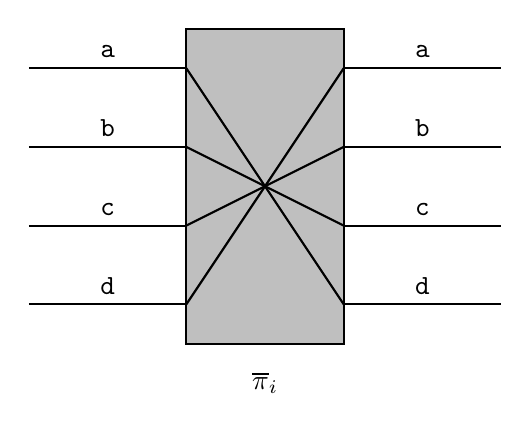
\begin{tikzpicture}[thick]
		% Draw the box
		\draw[fill=lightgray] (2,-1.5) rectangle (4,2.5) node[midway] {};

		\node at (3, -2) {$\overline\pi_i$};

		% Draw the wires entering the box
		\draw[-] (0, 2) -- (2, 2) node[midway, above] {\texttt{\texttt{a}}};
		\draw[-] (0, 1) -- (2, 1) node[midway, above] {\texttt{b}};
		\draw[-] (0, 0) -- (2, 0) node[midway, above] {\texttt{c}};
		\draw[-] (0,-1) -- (2,-1) node[midway, above] {\texttt{d}};

		% Draw the wires exiting the box with crossed mappings
		\draw[-] (4, 2) -- (6,2) node[midway, above] {\texttt{a}};
		\draw[-] (4, 1) -- (6, 1) node[midway, above] {\texttt{b}};
		\draw[-] (4, 0) -- (6, 0) node[midway, above] {\texttt{c}};
		\draw[-] (4,-1) -- (6, -1) node[midway, above] {\texttt{d}};

		% Draw the lines inside the box to represent the mapping
		\draw[-] (2, 2) -- (4,-1);
		\draw[-] (2, 1) -- (4, 0);
		\draw[-] (2, 0) -- (4, 1);
		\draw[-] (2,-1) -- (4, 2);

	\end{tikzpicture}
\end{center}
A couple quick notes about this abstraction. First as these lines are
simply wires, current can flow in either direction, left-to-right, or
right-to-left.
Second, we can apply current to multiple wires concurrently, for
example, applying current at $\texttt{a}$ and $\texttt{c}$ will cause
$\texttt{d}$ and $\texttt{b}$ to be
live on the other side of the machine.
Finally, the choice to use lower case letters will become clear
further in this section as we want to separate the plugboard letters
from the actual plaintext-ciphertext letters.
\\\\As described in our motivating example, we may want to connect
Engima permutations in series to capture an underlying relationship
between a plaintext-ciphertext pairing.
Suppose we had plaintext-ciphertext pairing
\begin{center}
	\begin{tikzpicture}[node distance=1cm, every node/.style={draw,
					circle, minimum height=0.1cm, minimum width=0.1cm}]

		% Centering the diagram
		\node (a1) [] {\texttt{B}};
		\node (a2) [right=0.1cm of a1] {\texttt{C}};
		\node (a3) [right=0.1cm of a2] {\texttt{A}};

		% Nodes for ciphertext
		\node (x1) [below=1cm of a1] {\texttt{A}};
		\node (x2) [below=1cm of a2] {\texttt{B}};
		\node (x3) [below=1cm of a3] {\texttt{C}};

		% Arrows for mapping
		\draw[->] (a1) -- (x1) node[midway, left, draw=none, fill=none] {1};
		\draw[->] (a2) -- (x2) node[midway, left, draw=none, fill=none] {2};
		\draw[->] (a3) -- (x3) node[midway, left, draw=none, fill=none] {3};

	\end{tikzpicture}
\end{center}

\noindent Then we find that there exists a loop in the pairing as follows

\begin{center}
	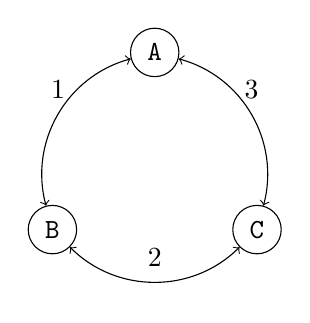
\begin{tikzpicture}[node distance=1cm, every node/.style={draw,
					circle, minimum height=0.1cm, minimum width=0.1cm}]
		\node (A) at (90:1.5) {\texttt{A}};
		\node (B) at (210:1.5) {\texttt{B}};
		\node (C) at (330:1.5) {\texttt{C}};

		\draw[<->, bend right=45] (A) to node[midway, draw=none, above] {1} (B);
		\draw[<->, bend right=45] (B) to node[midway, draw=none, above] {2} (C);
		\draw[<->, bend right=45] (C) to node[midway, draw=none, above] {3} (A);
	\end{tikzpicture}
\end{center}
We can then think of this loop as a series of three Enigma
permutations. We assume the message began with window setting
\texttt{ZZZ}. We will hypothesize some rotor ordering and we will
further assume a ring setting of \texttt{ZZZ}. Thus the first machine
will be set to a window setting \texttt{ZZZ}, the second set to
\texttt{ZZA}, and the third set to \texttt{ZZB}. Note that this is
assuming no turnover occured during our enciphering of the plaintext
-- a caveat we will later address. We can connect these Enigma
machines as follows
\begin{center}
	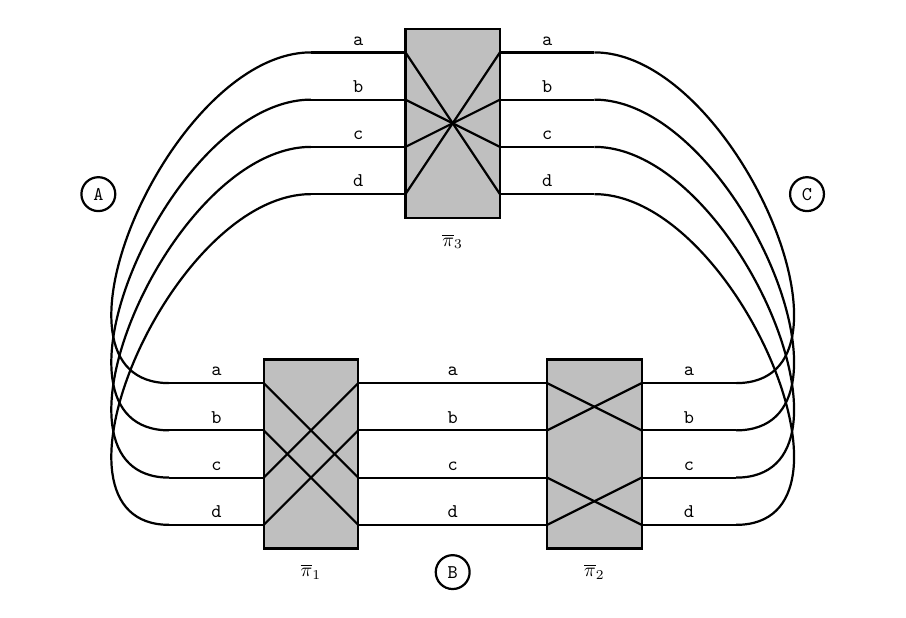
\begin{tikzpicture}[thick, scale=0.6, every node/.style={scale=0.7}]
		% Draw the box
		\draw[fill=lightgray] (2,-1.5) rectangle (4,2.5) node[midway] {};

		\node at (3, -2) {$\overline\pi_3$};

		% Draw the wires entering the box
		\draw[-] (0, 2) -- (2, 2) node[midway, above] {\texttt{a}};
		\draw[-] (0, 1) -- (2, 1) node[midway, above] {\texttt{b}};
		\draw[-] (0, 0) -- (2, 0) node[midway, above] {\texttt{c}};
		\draw[-] (0,-1) -- (2,-1) node[midway, above] {\texttt{d}};

		% Draw the wires exiting the box with crossed mappings
		\draw[-] (4, 2) -- (6,2) node[midway, above] {\texttt{a}};
		\draw[-] (4, 1) -- (6, 1) node[midway, above] {\texttt{b}};
		\draw[-] (4, 0) -- (6, 0) node[midway, above] {\texttt{c}};
		\draw[-] (4,-1) -- (6, -1) node[midway, above] {\texttt{d}};

		% Draw the lines inside the box to represent the mapping
		\draw[-] (2, 2) -- (4,-1);
		\draw[-] (2, 1) -- (4, 0);
		\draw[-] (2, 0) -- (4, 1);
		\draw[-] (2,-1) -- (4, 2);

		\draw[-] (0-3, 2-7) to[out=180, in=180] (0, 2) node[midway, above] {};
		\draw[-] (0-3, 1-7) to[out=180, in=180] (0, 1) node[midway, above] {};
		\draw[-] (0-3, 0-7) to[out=180, in=180] (0, 0) node[midway, above] {};
		\draw[-] (0-3, -1-7) to[out=180, in=180] (0, -1) node[midway, above] {};

		\draw[-] (6+3, 2-7) to[out=360, in=360] (6, 2) node[midway, above] {};
		\draw[-] (6+3, 1-7) to[out=360, in=360] (6, 1) node[midway, above] {};
		\draw[-] (6+3, 0-7) to[out=360, in=360] (6, 0) node[midway, above] {};
		\draw[-] (6+3, -1-7) to[out=360, in=360] (6, -1) node[midway, above] {};

		\draw[fill=lightgray] (2-3,-1.5-7) rectangle (4-3,2.5-7) node[midway] {};

		\node at (3-3, -2-7) {$\overline\pi_1$};

		% Draw the wires entering the box
		\draw[-] (0-3, 2-7) -- (2-3, 2-7) node[midway, above] {\texttt{a}};
		\draw[-] (0-3, 1-7) -- (2-3, 1-7) node[midway, above] {\texttt{b}};
		\draw[-] (0-3, 0-7) -- (2-3, 0-7) node[midway, above] {\texttt{c}};
		\draw[-] (0-3,-1-7) -- (2-3,-1-7) node[midway, above] {\texttt{d}};

		% Draw the wires exiting the box
		\draw[-] (4-3, 2-7) -- (6-3,2-7) node[right, above] {\texttt{a}};
		\draw[-] (4-3, 1-7) -- (6-3, 1-7) node[right, above] {\texttt{b}};
		\draw[-] (4-3, 0-7) -- (6-3, 0-7) node[right, above] {\texttt{c}};
		\draw[-] (4-3,-1-7) -- (6-3, -1-7) node[right, above] {\texttt{d}};

		% Draw the lines inside the box to represent the mapping
		\draw[-] (2-3, 2-7) -- (4-3, 0-7);
		\draw[-] (2-3, 1-7) -- (4-3, -1-7);
		\draw[-] (2-3, 0-7) -- (4-3, 2-7);
		\draw[-] (2-3,-1-7) -- (4-3, 1-7);

		\draw[fill=lightgray] (2+3,-1.5-7) rectangle (4+3,2.5-7) node[midway] {};

		\node at (3+3, -2-7) {$\overline\pi_2$};

		% Draw the wires entering the box
		\draw[-] (0+3, 2-7) -- (2+3, 2-7) node[midway, above] {};
		\draw[-] (0+3, 1-7) -- (2+3, 1-7) node[midway, above] {};
		\draw[-] (0+3, 0-7) -- (2+3, 0-7) node[midway, above] {};
		\draw[-] (0+3,-1-7) -- (2+3,-1-7) node[midway, above] {};

		% Draw the wires exiting the box
		\draw[-] (4+3, 2-7) -- (6+3,2-7) node[midway, above] {\texttt{a}};
		\draw[-] (4+3, 1-7) -- (6+3, 1-7) node[midway, above] {\texttt{b}};
		\draw[-] (4+3, 0-7) -- (6+3, 0-7) node[midway, above] {\texttt{c}};
		\draw[-] (4+3,-1-7) -- (6+3, -1-7) node[midway, above] {\texttt{d}};

		\draw[-] (2+3, 2-7) -- (4+3, 1-7);
		\draw[-] (2+3, 1-7) -- (4+3, 2-7);
		\draw[-] (2+3, 0-7) -- (4+3, -1-7);
		\draw[-] (2+3,-1-7) -- (4+3, 0-7);

		\node[draw,circle] at (-4.5, -1) {\texttt{A}};
		\node[draw,circle] at (3, -9) {\texttt{B}};
		\node[draw,circle] at (10.5, -1) {\texttt{C}};

	\end{tikzpicture}
\end{center}
As before, let us make a hypothesis regarding steckering. Suppose
$S(\texttt{A}) = \texttt{D}$. We know that $\texttt{A}$ must map to
$\texttt{A}$ via
$S^{-1}\overline\pi_3\overline\pi_2\overline\pi_1 S$. In our
diagram, however we do not see a plugboard so how can we represent
the plugboard's involvement? In order
to achieve this \emph{we} will function as the plugboard by applying
voltage to the $\texttt{d}$ line on the $\texttt{A}$ cable thus
implicitly performing the
plugboard mapping in which $S(\texttt{A}) = \texttt{D}$.
Then this will go through the electrical mapping $\overline\pi_1$
arriving on the \texttt{B} cable, followed by $\overline\pi_2$ arriving
on the \texttt{C} cable, followed by $\overline\pi_3$ arriving back on
the \texttt{A} cable, where \emph{we} as the implicit plugboard know that
the output of this electrical mapping must go through the plugboard
again to get a final output of \texttt{A}.
\\\\We will denote each wire by a capital and lowercase letter which
indicates both the cable and specific wire to which we refer. For
instance, line \texttt{d} on cable \texttt{A} will be denoted
$\texttt{Ad}$. Any time a wire
$\texttt{Xy}$ is live, implicitly this means that there is an intermediary
plugboard which mapped $S(\texttt{X}) = \texttt{Y}$ or $S(\texttt{Y})
	= \texttt{X}$.
To see this electrical mapping occur let us visualize a current being
sent through $\texttt{Ad}$.
\begin{figure}[H]
	\begin{minipage}{0.45\textwidth}
		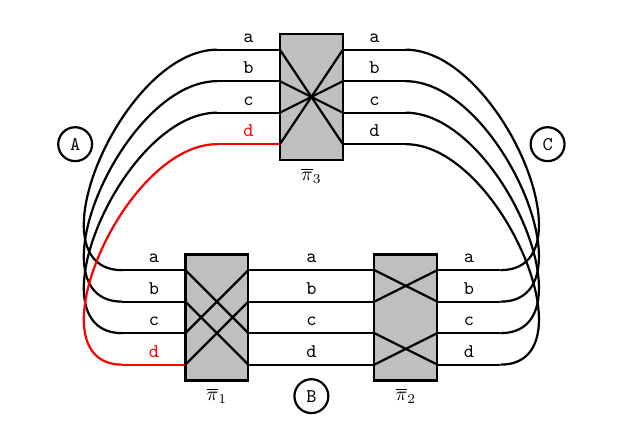
\begin{tikzpicture}[thick, scale=0.4, every node/.style={scale=0.7}]
			% Draw the box
			\draw[fill=lightgray] (2,-1.5) rectangle (4,2.5) node[midway] {};

			\node at (3, -2) {$\overline\pi_3$};

			% Draw the wires entering the box
			\draw[-] (0, 2) -- (2, 2) node[midway, above] {\texttt{a}};
			\draw[-] (0, 1) -- (2, 1) node[midway, above] {\texttt{b}};
			\draw[-] (0, 0) -- (2, 0) node[midway, above] {\texttt{c}};
			\draw[-, red] (0,-1) -- (2,-1) node[midway, above] {\texttt{d}};

			% Draw the wires exiting the box with crossed mappings
			\draw[-] (4, 2) -- (6,2) node[midway, above] {\texttt{a}};
			\draw[-] (4, 1) -- (6, 1) node[midway, above] {\texttt{b}};
			\draw[-] (4, 0) -- (6, 0) node[midway, above] {\texttt{c}};
			\draw[-] (4,-1) -- (6, -1) node[midway, above] {\texttt{d}};

			% Draw the lines inside the box to represent the mapping
			\draw[-] (2, 2) -- (4,-1);
			\draw[-] (2, 1) -- (4, 0);
			\draw[-] (2, 0) -- (4, 1);
			\draw[-] (2,-1) -- (4, 2);

			\draw[-] (0-3, 2-7) to[out=180, in=180] (0, 2) node[midway, above] {};
			\draw[-] (0-3, 1-7) to[out=180, in=180] (0, 1) node[midway, above] {};
			\draw[-] (0-3, 0-7) to[out=180, in=180] (0, 0) node[midway, above] {};
			\draw[-, red] (0-3, -1-7) to[out=180, in=180] (0, -1)
			node[midway, above] {};

			\draw[-] (6+3, 2-7) to[out=360, in=360] (6, 2) node[midway, above] {};
			\draw[-] (6+3, 1-7) to[out=360, in=360] (6, 1) node[midway, above] {};
			\draw[-] (6+3, 0-7) to[out=360, in=360] (6, 0) node[midway, above] {};
			\draw[-] (6+3, -1-7) to[out=360, in=360] (6, -1) node[midway, above] {};

			\draw[fill=lightgray] (2-3,-1.5-7) rectangle (4-3,2.5-7) node[midway] {};

			\node at (3-3, -2-7) {$\overline\pi_1$};

			% Draw the wires entering the box
			\draw[-] (0-3, 2-7) -- (2-3, 2-7) node[midway, above] {\texttt{a}};
			\draw[-] (0-3, 1-7) -- (2-3, 1-7) node[midway, above] {\texttt{b}};
			\draw[-] (0-3, 0-7) -- (2-3, 0-7) node[midway, above] {\texttt{c}};
			\draw[-, red] (0-3,-1-7) -- (2-3,-1-7) node[midway, above] {\texttt{d}};

			% Draw the wires exiting the box
			\draw[-] (4-3, 2-7) -- (6-3,2-7) node[right, above] {\texttt{a}};
			\draw[-] (4-3, 1-7) -- (6-3, 1-7) node[right, above] {\texttt{b}};
			\draw[-] (4-3, 0-7) -- (6-3, 0-7) node[right, above] {\texttt{c}};
			\draw[-] (4-3,-1-7) -- (6-3, -1-7) node[right, above] {\texttt{d}};

			% Draw the lines inside the box to represent the mapping
			\draw[-] (2-3, 2-7) -- (4-3, 0-7);
			\draw[-] (2-3, 1-7) -- (4-3, -1-7);
			\draw[-] (2-3, 0-7) -- (4-3, 2-7);
			\draw[-] (2-3,-1-7) -- (4-3, 1-7);

			\draw[fill=lightgray] (2+3,-1.5-7) rectangle (4+3,2.5-7) node[midway] {};

			\node at (3+3, -2-7) {$\overline\pi_2$};

			% Draw the wires entering the box
			\draw[-] (0+3, 2-7) -- (2+3, 2-7) node[midway, above] {};
			\draw[-] (0+3, 1-7) -- (2+3, 1-7) node[midway, above] {};
			\draw[-] (0+3, 0-7) -- (2+3, 0-7) node[midway, above] {};
			\draw[-] (0+3,-1-7) -- (2+3,-1-7) node[midway, above] {};

			% Draw the wires exiting the box
			\draw[-] (4+3, 2-7) -- (6+3,2-7) node[midway, above] {\texttt{a}};
			\draw[-] (4+3, 1-7) -- (6+3, 1-7) node[midway, above] {\texttt{b}};
			\draw[-] (4+3, 0-7) -- (6+3, 0-7) node[midway, above] {\texttt{c}};
			\draw[-] (4+3,-1-7) -- (6+3, -1-7) node[midway, above] {\texttt{d}};

			\draw[-] (2+3, 2-7) -- (4+3, 1-7);
			\draw[-] (2+3, 1-7) -- (4+3, 2-7);
			\draw[-] (2+3, 0-7) -- (4+3, -1-7);
			\draw[-] (2+3,-1-7) -- (4+3, 0-7);

			\node[draw,circle] at (-4.5, -1) {\texttt{A}};
			\node[draw,circle] at (3, -9) {\texttt{B}};
			\node[draw,circle] at (10.5, -1) {\texttt{C}};

		\end{tikzpicture}
	\end{minipage}
	\hfill
	\begin{minipage}{0.45\textwidth}
		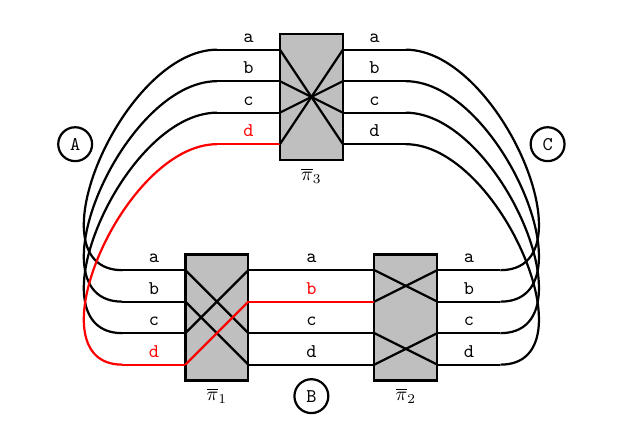
\begin{tikzpicture}[thick, scale=0.4, every node/.style={scale=0.7}]
			% Draw the box
			\draw[fill=lightgray] (2,-1.5) rectangle (4,2.5) node[midway] {};

			\node at (3, -2) {$\overline\pi_3$};

			% Draw the wires entering the box
			\draw[-] (0, 2) -- (2, 2) node[midway, above] {\texttt{a}};
			\draw[-] (0, 1) -- (2, 1) node[midway, above] {\texttt{b}};
			\draw[-] (0, 0) -- (2, 0) node[midway, above] {\texttt{c}};
			\draw[-, red] (0,-1) -- (2,-1) node[midway, above] {\texttt{d}};

			% Draw the wires exiting the box with crossed mappings
			\draw[-] (4, 2) -- (6,2) node[midway, above] {\texttt{a}};
			\draw[-] (4, 1) -- (6, 1) node[midway, above] {\texttt{b}};
			\draw[-] (4, 0) -- (6, 0) node[midway, above] {\texttt{c}};
			\draw[-] (4,-1) -- (6, -1) node[midway, above] {\texttt{d}};

			% Draw the lines inside the box to represent the mapping
			\draw[-] (2, 2) -- (4,-1);
			\draw[-] (2, 1) -- (4, 0);
			\draw[-] (2, 0) -- (4, 1);
			\draw[-] (2,-1) -- (4, 2);

			\draw[-] (0-3, 2-7) to[out=180, in=180] (0, 2) node[midway, above] {};
			\draw[-] (0-3, 1-7) to[out=180, in=180] (0, 1) node[midway, above] {};
			\draw[-] (0-3, 0-7) to[out=180, in=180] (0, 0) node[midway, above] {};
			\draw[-, red] (0-3, -1-7) to[out=180, in=180] (0, -1)
			node[midway, above] {};

			\draw[-] (6+3, 2-7) to[out=360, in=360] (6, 2) node[midway, above] {};
			\draw[-] (6+3, 1-7) to[out=360, in=360] (6, 1) node[midway, above] {};
			\draw[-] (6+3, 0-7) to[out=360, in=360] (6, 0) node[midway, above] {};
			\draw[-] (6+3, -1-7) to[out=360, in=360] (6, -1) node[midway, above] {};

			\draw[fill=lightgray] (2-3,-1.5-7) rectangle (4-3,2.5-7) node[midway] {};

			\node at (3-3, -2-7) {$\overline\pi_1$};

			% Draw the wires entering the box
			\draw[-] (0-3, 2-7) -- (2-3, 2-7) node[midway, above] {\texttt{a}};
			\draw[-] (0-3, 1-7) -- (2-3, 1-7) node[midway, above] {\texttt{b}};
			\draw[-] (0-3, 0-7) -- (2-3, 0-7) node[midway, above] {\texttt{c}};
			\draw[-, red] (0-3,-1-7) -- (2-3,-1-7) node[midway, above] {\texttt{d}};

			% Draw the wires exiting the box
			\draw[-] (4-3, 2-7) -- (6-3,2-7) node[right, above] {\texttt{a}};
			\draw[-, red] (4-3, 1-7) -- (6-3, 1-7) node[right, above] {\texttt{b}};
			\draw[-] (4-3, 0-7) -- (6-3, 0-7) node[right, above] {\texttt{c}};
			\draw[-] (4-3,-1-7) -- (6-3, -1-7) node[right, above] {\texttt{d}};

			% Draw the lines inside the box to represent the mapping
			\draw[-] (2-3, 2-7) -- (4-3, 0-7);
			\draw[-] (2-3, 1-7) -- (4-3, -1-7);
			\draw[-] (2-3, 0-7) -- (4-3, 2-7);
			\draw[-, red] (2-3,-1-7) -- (4-3, 1-7);

			\draw[fill=lightgray] (2+3,-1.5-7) rectangle (4+3,2.5-7) node[midway] {};

			\node at (3+3, -2-7) {$\overline\pi_2$};

			% Draw the wires entering the box
			\draw[-] (0+3, 2-7) -- (2+3, 2-7) node[midway, above] {};
			\draw[-, red] (0+3, 1-7) -- (2+3, 1-7) node[midway, above] {};
			\draw[-] (0+3, 0-7) -- (2+3, 0-7) node[midway, above] {};
			\draw[-] (0+3,-1-7) -- (2+3,-1-7) node[midway, above] {};

			% Draw the wires exiting the box
			\draw[-] (4+3, 2-7) -- (6+3,2-7) node[midway, above] {\texttt{a}};
			\draw[-] (4+3, 1-7) -- (6+3, 1-7) node[midway, above] {\texttt{b}};
			\draw[-] (4+3, 0-7) -- (6+3, 0-7) node[midway, above] {\texttt{c}};
			\draw[-] (4+3,-1-7) -- (6+3, -1-7) node[midway, above] {\texttt{d}};

			\draw[-] (2+3, 2-7) -- (4+3, 1-7);
			\draw[-] (2+3, 1-7) -- (4+3, 2-7);
			\draw[-] (2+3, 0-7) -- (4+3, -1-7);
			\draw[-] (2+3,-1-7) -- (4+3, 0-7);

			\node[draw,circle] at (-4.5, -1) {\texttt{A}};
			\node[draw,circle] at (3, -9) {\texttt{B}};
			\node[draw,circle] at (10.5, -1) {\texttt{C}};

		\end{tikzpicture}
	\end{minipage}
	\\\\\\\\
	\noindent
	\begin{minipage}{0.45\textwidth}
		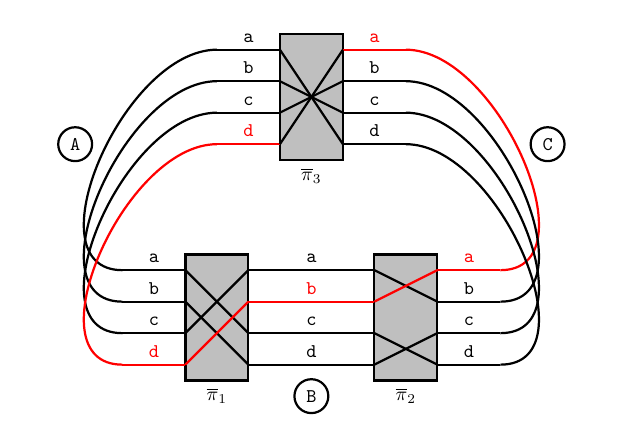
\begin{tikzpicture}[thick, scale=0.4, every node/.style={scale=0.7}]
			% Draw the box
			\draw[fill=lightgray] (2,-1.5) rectangle (4,2.5) node[midway] {};

			\node at (3, -2) {$\overline\pi_3$};

			% Draw the wires entering the box
			\draw[-] (0, 2) -- (2, 2) node[midway, above] {\texttt{a}};
			\draw[-] (0, 1) -- (2, 1) node[midway, above] {\texttt{b}};
			\draw[-] (0, 0) -- (2, 0) node[midway, above] {\texttt{c}};
			\draw[-, red] (0,-1) -- (2,-1) node[midway, above] {\texttt{d}};

			% Draw the wires exiting the box with crossed mappings
			\draw[-, red] (4, 2) -- (6,2) node[midway, above] {\texttt{a}};
			\draw[-] (4, 1) -- (6, 1) node[midway, above] {\texttt{b}};
			\draw[-] (4, 0) -- (6, 0) node[midway, above] {\texttt{c}};
			\draw[-] (4,-1) -- (6, -1) node[midway, above] {\texttt{d}};

			% Draw the lines inside the box to represent the mapping
			\draw[-] (2, 2) -- (4,-1);
			\draw[-] (2, 1) -- (4, 0);
			\draw[-] (2, 0) -- (4, 1);
			\draw[-] (2,-1) -- (4, 2);

			\draw[-] (0-3, 2-7) to[out=180, in=180] (0, 2) node[midway, above] {};
			\draw[-] (0-3, 1-7) to[out=180, in=180] (0, 1) node[midway, above] {};
			\draw[-] (0-3, 0-7) to[out=180, in=180] (0, 0) node[midway, above] {};
			\draw[-, red] (0-3, -1-7) to[out=180, in=180] (0, -1)
			node[midway, above] {};

			\draw[- ,red] (6+3, 2-7) to[out=360, in=360] (6, 2)
			node[midway, above] {};
			\draw[-] (6+3, 1-7) to[out=360, in=360] (6, 1) node[midway, above] {};
			\draw[-] (6+3, 0-7) to[out=360, in=360] (6, 0) node[midway, above] {};
			\draw[-] (6+3, -1-7) to[out=360, in=360] (6, -1) node[midway, above] {};

			\draw[fill=lightgray] (2-3,-1.5-7) rectangle (4-3,2.5-7) node[midway] {};

			\node at (3-3, -2-7) {$\overline\pi_1$};

			% Draw the wires entering the box
			\draw[-] (0-3, 2-7) -- (2-3, 2-7) node[midway, above] {\texttt{a}};
			\draw[-] (0-3, 1-7) -- (2-3, 1-7) node[midway, above] {\texttt{b}};
			\draw[-] (0-3, 0-7) -- (2-3, 0-7) node[midway, above] {\texttt{c}};
			\draw[-, red] (0-3,-1-7) -- (2-3,-1-7) node[midway, above] {\texttt{d}};

			% Draw the wires exiting the box
			\draw[-] (4-3, 2-7) -- (6-3,2-7) node[right, above] {\texttt{a}};
			\draw[-, red] (4-3, 1-7) -- (6-3, 1-7) node[right, above] {\texttt{b}};
			\draw[-] (4-3, 0-7) -- (6-3, 0-7) node[right, above] {\texttt{c}};
			\draw[-] (4-3,-1-7) -- (6-3, -1-7) node[right, above] {\texttt{d}};

			% Draw the lines inside the box to represent the mapping
			\draw[-] (2-3, 2-7) -- (4-3, 0-7);
			\draw[-] (2-3, 1-7) -- (4-3, -1-7);
			\draw[-] (2-3, 0-7) -- (4-3, 2-7);
			\draw[-, red] (2-3,-1-7) -- (4-3, 1-7);

			\draw[fill=lightgray] (2+3,-1.5-7) rectangle (4+3,2.5-7) node[midway] {};

			\node at (3+3, -2-7) {$\overline\pi_2$};

			% Draw the wires entering the box
			\draw[-] (0+3, 2-7) -- (2+3, 2-7) node[midway, above] {};
			\draw[-, red] (0+3, 1-7) -- (2+3, 1-7) node[midway, above] {};
			\draw[-] (0+3, 0-7) -- (2+3, 0-7) node[midway, above] {};
			\draw[-] (0+3,-1-7) -- (2+3,-1-7) node[midway, above] {};

			% Draw the wires exiting the box
			\draw[-, red] (4+3, 2-7) -- (6+3,2-7) node[midway, above] {\texttt{a}};
			\draw[-] (4+3, 1-7) -- (6+3, 1-7) node[midway, above] {\texttt{b}};
			\draw[-] (4+3, 0-7) -- (6+3, 0-7) node[midway, above] {\texttt{c}};
			\draw[-] (4+3,-1-7) -- (6+3, -1-7) node[midway, above] {\texttt{d}};

			\draw[-] (2+3, 2-7) -- (4+3, 1-7);
			\draw[-, red] (2+3, 1-7) -- (4+3, 2-7);
			\draw[-] (2+3, 0-7) -- (4+3, -1-7);
			\draw[-] (2+3,-1-7) -- (4+3, 0-7);

			\node[draw,circle] at (-4.5, -1) {\texttt{A}};
			\node[draw,circle] at (3, -9) {\texttt{B}};
			\node[draw,circle] at (10.5, -1) {\texttt{C}};

		\end{tikzpicture}
	\end{minipage}
	\hfill
	\begin{minipage}{0.45\textwidth}
		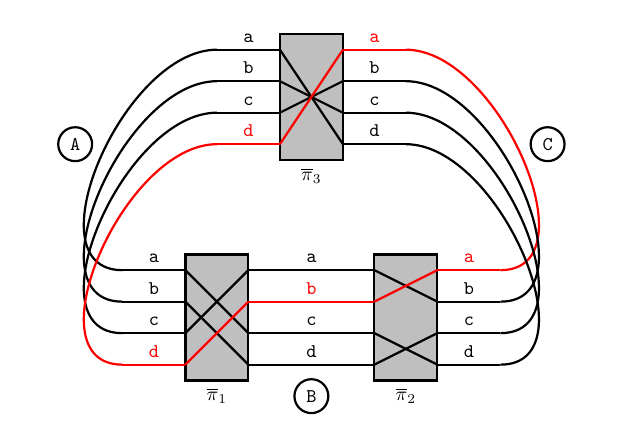
\begin{tikzpicture}[thick, scale=0.4, every node/.style={scale=0.7}]
			% Draw the box
			\draw[fill=lightgray] (2,-1.5) rectangle (4,2.5) node[midway] {};

			\node at (3, -2) {$\overline\pi_3$};

			% Draw the wires entering the box
			\draw[-] (0, 2) -- (2, 2) node[midway, above] {\texttt{a}};
			\draw[-] (0, 1) -- (2, 1) node[midway, above] {\texttt{b}};
			\draw[-] (0, 0) -- (2, 0) node[midway, above] {\texttt{c}};
			\draw[-, red] (0,-1) -- (2,-1) node[midway, above] {\texttt{d}};

			% Draw the wires exiting the box with crossed mappings
			\draw[-, red] (4, 2) -- (6,2) node[midway, above] {\texttt{a}};
			\draw[-] (4, 1) -- (6, 1) node[midway, above] {\texttt{b}};
			\draw[-] (4, 0) -- (6, 0) node[midway, above] {\texttt{c}};
			\draw[-] (4,-1) -- (6, -1) node[midway, above] {\texttt{d}};

			% Draw the lines inside the box to represent the mapping
			\draw[-] (2, 2) -- (4,-1);
			\draw[-] (2, 1) -- (4, 0);
			\draw[-] (2, 0) -- (4, 1);
			\draw[-, red] (2,-1) -- (4, 2);

			\draw[-] (0-3, 2-7) to[out=180, in=180] (0, 2) node[midway, above] {};
			\draw[-] (0-3, 1-7) to[out=180, in=180] (0, 1) node[midway, above] {};
			\draw[-] (0-3, 0-7) to[out=180, in=180] (0, 0) node[midway, above] {};
			\draw[-, red] (0-3, -1-7) to[out=180, in=180] (0, -1)
			node[midway, above] {};

			\draw[- ,red] (6+3, 2-7) to[out=360, in=360] (6, 2)
			node[midway, above] {};
			\draw[-] (6+3, 1-7) to[out=360, in=360] (6, 1) node[midway, above] {};
			\draw[-] (6+3, 0-7) to[out=360, in=360] (6, 0) node[midway, above] {};
			\draw[-] (6+3, -1-7) to[out=360, in=360] (6, -1) node[midway, above] {};

			\draw[fill=lightgray] (2-3,-1.5-7) rectangle (4-3,2.5-7) node[midway] {};

			\node at (3-3, -2-7) {$\overline\pi_1$};

			% Draw the wires entering the box
			\draw[-] (0-3, 2-7) -- (2-3, 2-7) node[midway, above] {\texttt{a}};
			\draw[-] (0-3, 1-7) -- (2-3, 1-7) node[midway, above] {\texttt{b}};
			\draw[-] (0-3, 0-7) -- (2-3, 0-7) node[midway, above] {\texttt{c}};
			\draw[-, red] (0-3,-1-7) -- (2-3,-1-7) node[midway, above] {\texttt{d}};

			% Draw the wires exiting the box
			\draw[-] (4-3, 2-7) -- (6-3,2-7) node[right, above] {\texttt{a}};
			\draw[-, red] (4-3, 1-7) -- (6-3, 1-7) node[right, above] {\texttt{b}};
			\draw[-] (4-3, 0-7) -- (6-3, 0-7) node[right, above] {\texttt{c}};
			\draw[-] (4-3,-1-7) -- (6-3, -1-7) node[right, above] {\texttt{d}};

			% Draw the lines inside the box to represent the mapping
			\draw[-] (2-3, 2-7) -- (4-3, 0-7);
			\draw[-] (2-3, 1-7) -- (4-3, -1-7);
			\draw[-] (2-3, 0-7) -- (4-3, 2-7);
			\draw[-, red] (2-3,-1-7) -- (4-3, 1-7);

			\draw[fill=lightgray] (2+3,-1.5-7) rectangle (4+3,2.5-7) node[midway] {};

			\node at (3+3, -2-7) {$\overline\pi_2$};

			% Draw the wires entering the box
			\draw[-] (0+3, 2-7) -- (2+3, 2-7) node[midway, above] {};
			\draw[-, red] (0+3, 1-7) -- (2+3, 1-7) node[midway, above] {};
			\draw[-] (0+3, 0-7) -- (2+3, 0-7) node[midway, above] {};
			\draw[-] (0+3,-1-7) -- (2+3,-1-7) node[midway, above] {};

			% Draw the wires exiting the box
			\draw[-, red] (4+3, 2-7) -- (6+3,2-7) node[midway, above] {\texttt{a}};
			\draw[-] (4+3, 1-7) -- (6+3, 1-7) node[midway, above] {\texttt{b}};
			\draw[-] (4+3, 0-7) -- (6+3, 0-7) node[midway, above] {\texttt{c}};
			\draw[-] (4+3,-1-7) -- (6+3, -1-7) node[midway, above] {\texttt{d}};

			\draw[-] (2+3, 2-7) -- (4+3, 1-7);
			\draw[-, red] (2+3, 1-7) -- (4+3, 2-7);
			\draw[-] (2+3, 0-7) -- (4+3, -1-7);
			\draw[-] (2+3,-1-7) -- (4+3, 0-7);

			\node[draw,circle] at (-4.5, -1) {\texttt{A}};
			\node[draw,circle] at (3, -9) {\texttt{B}};
			\node[draw,circle] at (10.5, -1) {\texttt{C}};

		\end{tikzpicture}
	\end{minipage}
	\caption{Current passing from wire \texttt{Ad} back to wire \texttt{Ad}}
	\label{fig:correct_stecker}
\end{figure}
\noindent Following our hypothesis that $S(\texttt{A}) = \texttt{D}$
we find that after sending
current through $\texttt{Ad}$ we arrive after mapping through
$\overline\pi$ back at $\texttt{Ad}$. Since we got an output of
$\texttt{D}$ before the plugboard mapping, and we know that at the
end this will ultimately map back through the plugboard to
$\texttt{A}$ in order preserve our fixed point at $\texttt{A}$, we
get the statement that $S(\texttt{D}) = \texttt{A}$ which is
perfectly consistent with our original hypothesis.
\\\\On the other hand, if we change
$\overline\pi$ and repeat this process which may end up in the
following situation
\begin{figure}[H]
	\begin{minipage}{0.45\textwidth}
		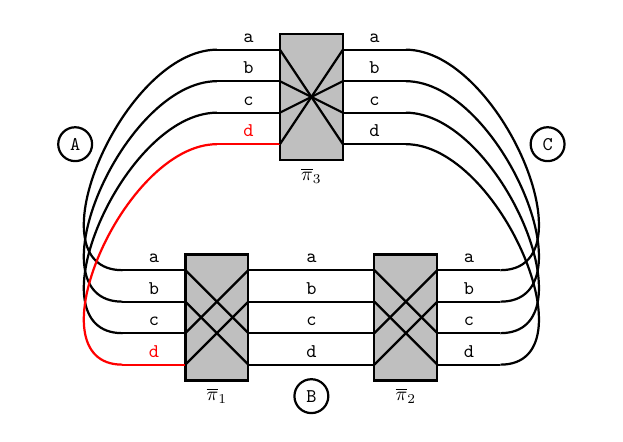
\begin{tikzpicture}[thick, scale=0.4, every node/.style={scale=0.7}]
			% Draw the box
			\draw[fill=lightgray] (2,-1.5) rectangle (4,2.5) node[midway] {};

			\node at (3, -2) {$\overline\pi_3$};

			% Draw the wires entering the box
			\draw[-] (0, 2) -- (2, 2) node[midway, above] {\texttt{a}};
			\draw[-] (0, 1) -- (2, 1) node[midway, above] {\texttt{b}};
			\draw[-] (0, 0) -- (2, 0) node[midway, above] {\texttt{c}};
			\draw[-, red] (0,-1) -- (2,-1) node[midway, above] {\texttt{d}};

			% Draw the wires exiting the box with crossed mappings
			\draw[-] (4, 2) -- (6,2) node[midway, above] {\texttt{a}};
			\draw[-] (4, 1) -- (6, 1) node[midway, above] {\texttt{b}};
			\draw[-] (4, 0) -- (6, 0) node[midway, above] {\texttt{c}};
			\draw[-] (4,-1) -- (6, -1) node[midway, above] {\texttt{d}};

			% Draw the lines inside the box to represent the mapping
			\draw[-] (2, 2) -- (4,-1);
			\draw[-] (2, 1) -- (4, 0);
			\draw[-] (2, 0) -- (4, 1);
			\draw[-] (2,-1) -- (4, 2);

			\draw[-] (0-3, 2-7) to[out=180, in=180] (0, 2) node[midway, above] {};
			\draw[-] (0-3, 1-7) to[out=180, in=180] (0, 1) node[midway, above] {};
			\draw[-] (0-3, 0-7) to[out=180, in=180] (0, 0) node[midway, above] {};
			\draw[-, red] (0-3, -1-7) to[out=180, in=180] (0, -1)
			node[midway, above] {};

			\draw[-] (6+3, 2-7) to[out=360, in=360] (6, 2) node[midway, above] {};
			\draw[-] (6+3, 1-7) to[out=360, in=360] (6, 1) node[midway, above] {};
			\draw[-] (6+3, 0-7) to[out=360, in=360] (6, 0) node[midway, above] {};
			\draw[-] (6+3, -1-7) to[out=360, in=360] (6, -1) node[midway, above] {};

			\draw[fill=lightgray] (2-3,-1.5-7) rectangle (4-3,2.5-7) node[midway] {};

			\node at (3-3, -2-7) {$\overline\pi_1$};

			% Draw the wires entering the box
			\draw[-] (0-3, 2-7) -- (2-3, 2-7) node[midway, above] {\texttt{a}};
			\draw[-] (0-3, 1-7) -- (2-3, 1-7) node[midway, above] {\texttt{b}};
			\draw[-] (0-3, 0-7) -- (2-3, 0-7) node[midway, above] {\texttt{c}};
			\draw[-, red] (0-3,-1-7) -- (2-3,-1-7) node[midway, above] {\texttt{d}};

			% Draw the wires exiting the box
			\draw[-] (4-3, 2-7) -- (6-3,2-7) node[right, above] {\texttt{a}};
			\draw[-] (4-3, 1-7) -- (6-3, 1-7) node[right, above] {\texttt{b}};
			\draw[-] (4-3, 0-7) -- (6-3, 0-7) node[right, above] {\texttt{c}};
			\draw[-] (4-3,-1-7) -- (6-3, -1-7) node[right, above] {\texttt{d}};

			% Draw the lines inside the box to represent the mapping
			\draw[-] (2-3, 2-7) -- (4-3, 0-7);
			\draw[-] (2-3, 1-7) -- (4-3, -1-7);
			\draw[-] (2-3, 0-7) -- (4-3, 2-7);
			\draw[-] (2-3,-1-7) -- (4-3, 1-7);

			\draw[fill=lightgray] (2+3,-1.5-7) rectangle (4+3,2.5-7) node[midway] {};

			\node at (3+3, -2-7) {$\overline\pi_2$};

			% Draw the wires entering the box
			\draw[-] (0+3, 2-7) -- (2+3, 2-7) node[midway, above] {};
			\draw[-] (0+3, 1-7) -- (2+3, 1-7) node[midway, above] {};
			\draw[-] (0+3, 0-7) -- (2+3, 0-7) node[midway, above] {};
			\draw[-] (0+3,-1-7) -- (2+3,-1-7) node[midway, above] {};

			% Draw the wires exiting the box
			\draw[-] (4+3, 2-7) -- (6+3,2-7) node[midway, above] {\texttt{a}};
			\draw[-] (4+3, 1-7) -- (6+3, 1-7) node[midway, above] {\texttt{b}};
			\draw[-] (4+3, 0-7) -- (6+3, 0-7) node[midway, above] {\texttt{c}};
			\draw[-] (4+3,-1-7) -- (6+3, -1-7) node[midway, above] {\texttt{d}};

			\draw[-] (2+3, 2-7) -- (4+3, 0-7);
			\draw[-] (2+3, 1-7) -- (4+3, -1-7);
			\draw[-] (2+3, 0-7) -- (4+3, 2-7);
			\draw[-] (2+3,-1-7) -- (4+3, 1-7);

			\node[draw,circle] at (-4.5, -1) {\texttt{\texttt{A}}};
			\node[draw,circle] at (3, -9) {\texttt{\texttt{B}}};
			\node[draw,circle] at (10.5, -1) {\texttt{\texttt{C}}};

		\end{tikzpicture}
	\end{minipage}
	\hfill
	\begin{minipage}{0.45\textwidth}
		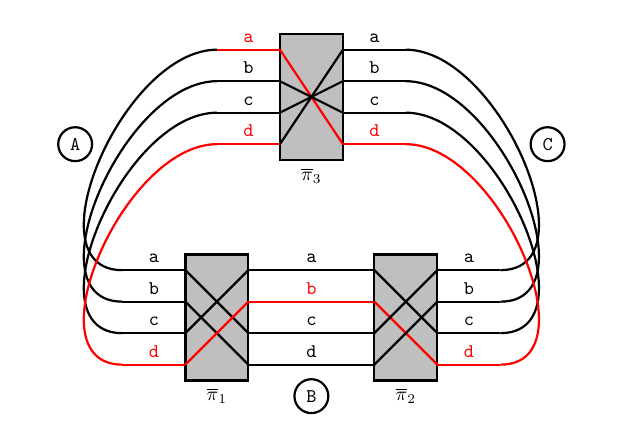
\begin{tikzpicture}[thick, scale=0.4, every node/.style={scale=0.7}]
			% Draw the box
			\draw[fill=lightgray] (2,-1.5) rectangle (4,2.5) node[midway] {};

			\node at (3, -2) {$\overline\pi_3$};

			% Draw the wires entering the box
			\draw[-, red] (0, 2) -- (2, 2) node[midway, above] {\texttt{a}};
			\draw[-] (0, 1) -- (2, 1) node[midway, above] {\texttt{b}};
			\draw[-] (0, 0) -- (2, 0) node[midway, above] {\texttt{c}};
			\draw[-, red] (0,-1) -- (2,-1) node[midway, above] {\texttt{d}};

			% Draw the wires exiting the box with crossed mappings
			\draw[-] (4, 2) -- (6,2) node[midway, above] {\texttt{a}};
			\draw[-] (4, 1) -- (6, 1) node[midway, above] {\texttt{b}};
			\draw[-] (4, 0) -- (6, 0) node[midway, above] {\texttt{c}};
			\draw[-, red] (4,-1) -- (6, -1) node[midway, above] {\texttt{d}};

			% Draw the lines inside the box to represent the mapping
			\draw[-, red] (2, 2) -- (4,-1);
			\draw[-] (2, 1) -- (4, 0);
			\draw[-] (2, 0) -- (4, 1);
			\draw[-] (2,-1) -- (4, 2);

			\draw[-] (0-3, 2-7) to[out=180, in=180] (0, 2) node[midway, above] {};
			\draw[-] (0-3, 1-7) to[out=180, in=180] (0, 1) node[midway, above] {};
			\draw[-] (0-3, 0-7) to[out=180, in=180] (0, 0) node[midway, above] {};
			\draw[-, red] (0-3, -1-7) to[out=180, in=180] (0, -1)
			node[midway, above] {};

			\draw[-] (6+3, 2-7) to[out=360, in=360] (6, 2) node[midway, above] {};
			\draw[-] (6+3, 1-7) to[out=360, in=360] (6, 1) node[midway, above] {};
			\draw[-] (6+3, 0-7) to[out=360, in=360] (6, 0) node[midway, above] {};
			\draw[-, red] (6+3, -1-7) to[out=360, in=360] (6, -1)
			node[midway, above] {};

			\draw[fill=lightgray] (2-3,-1.5-7) rectangle (4-3,2.5-7) node[midway] {};

			\node at (3-3, -2-7) {$\overline\pi_1$};

			% Draw the wires entering the box
			\draw[-] (0-3, 2-7) -- (2-3, 2-7) node[midway, above] {\texttt{a}};
			\draw[-] (0-3, 1-7) -- (2-3, 1-7) node[midway, above] {\texttt{b}};
			\draw[-] (0-3, 0-7) -- (2-3, 0-7) node[midway, above] {\texttt{c}};
			\draw[-, red] (0-3,-1-7) -- (2-3,-1-7) node[midway, above] {\texttt{d}};

			% Draw the wires exiting the box
			\draw[-] (4-3, 2-7) -- (6-3,2-7) node[right, above] {\texttt{a}};
			\draw[-, red] (4-3, 1-7) -- (6-3, 1-7) node[right, above] {\texttt{b}};
			\draw[-] (4-3, 0-7) -- (6-3, 0-7) node[right, above] {\texttt{c}};
			\draw[-] (4-3,-1-7) -- (6-3, -1-7) node[right, above] {\texttt{d}};

			% Draw the lines inside the box to represent the mapping
			\draw[-] (2-3, 2-7) -- (4-3, 0-7);
			\draw[-] (2-3, 1-7) -- (4-3, -1-7);
			\draw[-] (2-3, 0-7) -- (4-3, 2-7);
			\draw[-, red] (2-3,-1-7) -- (4-3, 1-7);

			\draw[fill=lightgray] (2+3,-1.5-7) rectangle (4+3,2.5-7) node[midway] {};

			\node at (3+3, -2-7) {$\overline\pi_2$};

			% Draw the wires entering the box
			\draw[-] (0+3, 2-7) -- (2+3, 2-7) node[midway, above] {};
			\draw[-, red] (0+3, 1-7) -- (2+3, 1-7) node[midway, above] {};
			\draw[-] (0+3, 0-7) -- (2+3, 0-7) node[midway, above] {};
			\draw[-] (0+3,-1-7) -- (2+3,-1-7) node[midway, above] {};

			% Draw the wires exiting the box
			\draw[-] (4+3, 2-7) -- (6+3,2-7) node[midway, above] {\texttt{a}};
			\draw[-] (4+3, 1-7) -- (6+3, 1-7) node[midway, above] {\texttt{b}};
			\draw[-] (4+3, 0-7) -- (6+3, 0-7) node[midway, above] {\texttt{c}};
			\draw[-, red] (4+3,-1-7) -- (6+3, -1-7) node[midway, above] {\texttt{d}};

			\draw[-] (2+3, 2-7) -- (4+3, 0-7);
			\draw[-, red] (2+3, 1-7) -- (4+3, -1-7);
			\draw[-] (2+3, 0-7) -- (4+3, 2-7);
			\draw[-] (2+3,-1-7) -- (4+3, 1-7);

			\node[draw,circle] at (-4.5, -1) {\texttt{\texttt{A}}};
			\node[draw,circle] at (3, -9) {\texttt{\texttt{B}}};
			\node[draw,circle] at (10.5, -1) {\texttt{\texttt{C}}};

		\end{tikzpicture}
	\end{minipage}
	\caption{Current passing from wire \texttt{Ad} ending up at wire \texttt{Aa}}
	\label{fig:incorrect_stecker}
\end{figure}
\noindent In this example, following our steckering hypothesis
$S(\texttt{A}) = \texttt{D}$,
results in \texttt{Aa} becoming live after mapping through $\overline\pi$ and
thus we must have $S(\texttt{A}) = \texttt{A}$ as well in order for
this to ultimately
map back to \texttt{A} and preserve our fixed point at \texttt{A}.
This creates an inconsistency between our hypothesis and deduction
meaning that we can eliminate the steckering possibilities both
steckering possibilities so that $S(\texttt{A}) \notin \{\texttt{A},
	\texttt{D}\}$
\\\\Effectively, this process is a mechanization of
finding the cycle containing a particular letter. In the above
figure~\ref{fig:incorrect_stecker} sending current from \texttt{Ad}
until we arrive back at \texttt{Ad} is
akin to repeatedly applying $\overline\pi$ to \texttt{D}
until we return to \texttt{D}. This can be visualized in our diagram as

\begin{center}
	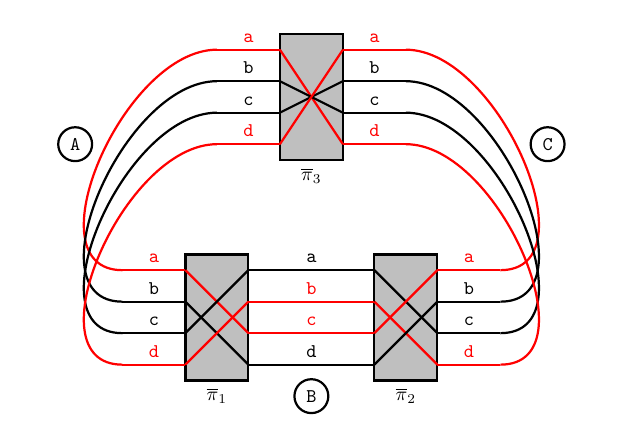
\begin{tikzpicture}[thick, scale=0.4, every node/.style={scale=0.7}]
		% Draw the box
		\draw[fill=lightgray] (2,-1.5) rectangle (4,2.5) node[midway] {};

		\node at (3, -2) {$\overline\pi_3$};

		% Draw the wires entering the box
		\draw[-, red] (0, 2) -- (2, 2) node[midway, above] {\texttt{a}};
		\draw[-] (0, 1) -- (2, 1) node[midway, above] {\texttt{b}};
		\draw[-] (0, 0) -- (2, 0) node[midway, above] {\texttt{c}};
		\draw[-, red] (0,-1) -- (2,-1) node[midway, above] {\texttt{d}};

		% Draw the wires exiting the box with crossed mappings
		\draw[-, red] (4, 2) -- (6,2) node[midway, above] {\texttt{a}};
		\draw[-] (4, 1) -- (6, 1) node[midway, above] {\texttt{b}};
		\draw[-] (4, 0) -- (6, 0) node[midway, above] {\texttt{c}};
		\draw[-, red] (4,-1) -- (6, -1) node[midway, above] {\texttt{d}};

		% Draw the lines inside the box to represent the mapping
		\draw[-, red] (2, 2) -- (4,-1);
		\draw[-] (2, 1) -- (4, 0);
		\draw[-] (2, 0) -- (4, 1);
		\draw[-, red] (2,-1) -- (4, 2);

		\draw[-, red] (0-3, 2-7) to[out=180, in=180] (0, 2) node[midway, above] {};
		\draw[-] (0-3, 1-7) to[out=180, in=180] (0, 1) node[midway, above] {};
		\draw[-] (0-3, 0-7) to[out=180, in=180] (0, 0) node[midway, above] {};
		\draw[-, red] (0-3, -1-7) to[out=180, in=180] (0, -1)
		node[midway, above] {};

		\draw[-, red] (6+3, 2-7) to[out=360, in=360] (6, 2) node[midway, above] {};
		\draw[-] (6+3, 1-7) to[out=360, in=360] (6, 1) node[midway, above] {};
		\draw[-] (6+3, 0-7) to[out=360, in=360] (6, 0) node[midway, above] {};
		\draw[-, red] (6+3, -1-7) to[out=360, in=360] (6, -1)
		node[midway, above] {};

		\draw[fill=lightgray] (2-3,-1.5-7) rectangle (4-3,2.5-7) node[midway] {};

		\node at (3-3, -2-7) {$\overline\pi_1$};

		% Draw the wires entering the box
		\draw[-, red] (0-3, 2-7) -- (2-3, 2-7) node[midway, above] {\texttt{a}};
		\draw[-] (0-3, 1-7) -- (2-3, 1-7) node[midway, above] {\texttt{b}};
		\draw[-] (0-3, 0-7) -- (2-3, 0-7) node[midway, above] {\texttt{c}};
		\draw[-, red] (0-3,-1-7) -- (2-3,-1-7) node[midway, above] {\texttt{d}};

		% Draw the wires exiting the box
		\draw[-] (4-3, 2-7) -- (6-3,2-7) node[right, above] {\texttt{a}};
		\draw[-, red] (4-3, 1-7) -- (6-3, 1-7) node[right, above] {\texttt{b}};
		\draw[-, red] (4-3, 0-7) -- (6-3, 0-7) node[right, above] {\texttt{c}};
		\draw[-] (4-3,-1-7) -- (6-3, -1-7) node[right, above] {\texttt{d}};

		% Draw the lines inside the box to represent the mapping
		\draw[-, red] (2-3, 2-7) -- (4-3, 0-7);
		\draw[-] (2-3, 1-7) -- (4-3, -1-7);
		\draw[-] (2-3, 0-7) -- (4-3, 2-7);
		\draw[-, red] (2-3,-1-7) -- (4-3, 1-7);

		\draw[fill=lightgray] (2+3,-1.5-7) rectangle (4+3,2.5-7) node[midway] {};

		\node at (3+3, -2-7) {$\overline\pi_2$};

		% Draw the wires entering the box
		\draw[-] (0+3, 2-7) -- (2+3, 2-7) node[midway, above] {};
		\draw[-, red] (0+3, 1-7) -- (2+3, 1-7) node[midway, above] {};
		\draw[-, red] (0+3, 0-7) -- (2+3, 0-7) node[midway, above] {};
		\draw[-] (0+3,-1-7) -- (2+3,-1-7) node[midway, above] {};

		% Draw the wires exiting the box
		\draw[-, red] (4+3, 2-7) -- (6+3,2-7) node[midway, above] {\texttt{a}};
		\draw[-] (4+3, 1-7) -- (6+3, 1-7) node[midway, above] {\texttt{b}};
		\draw[-] (4+3, 0-7) -- (6+3, 0-7) node[midway, above] {\texttt{c}};
		\draw[-, red] (4+3,-1-7) -- (6+3, -1-7) node[midway, above] {\texttt{d}};

		\draw[-] (2+3, 2-7) -- (4+3, 0-7);
		\draw[-, red] (2+3, 1-7) -- (4+3, -1-7);
		\draw[-, red] (2+3, 0-7) -- (4+3, 2-7);
		\draw[-] (2+3,-1-7) -- (4+3, 1-7);

		\node[draw,circle] at (-4.5, -1) {\texttt{A}};
		\node[draw,circle] at (3, -9) {\texttt{B}};
		\node[draw,circle] at (10.5, -1) {\texttt{C}};

	\end{tikzpicture}
\end{center}
Where we find that in $\overline\pi$ we have the cycle $(\texttt{AD})$
since \texttt{Ad} and \texttt{Aa} are the only two live
wires in the \texttt{A} cable after allowing currently to reach a
steady-state. If we had instead applied current to \texttt{Ab} we would find
that \texttt{Ab} and \texttt{Ac} become live and give us the full
permutation $\overline\pi = (\texttt{AD})(\texttt{BC})$. The beauty
of this design
is that it is able to deduce the elements in a cycle of
$\overline\pi$ nearly instantaneously since it only requires the
circuit to reach
a steady-state.
\\\\Equipped with this tool spider-scanning becomes quite trivial.
The goal of spider-scanning is to eliminate a rotor position by
checking if the permutation has a $26$-cycle. In our diagram, with four lines,
this would be analogous to testing a steckering hypothesis (any
hypothesis) and finding that the entire cable becomes live. Then all
elements lie within the same cycle of $\overline\pi$ and thus all
steckering possibilities are immediately eliminated.
\\\\The Bombe is designed to quickly move through all $26^3$ possible
window settings while maintaining the same relative distances between
each Enigma permutation in our loop. At each configuration
it applies current to test our steckering hypothesis and, only when
an arrangement is such that it
cannot be eliminated and further examination is needed, we will cause
the machine to stop.

\subsubsection{Scramblers}
Thus far we have described the Bombe as connecting Enigma machines.
In reality, the Bombe used a set of rotors known as {\bf{drums}}
mimicking the effect of each Enigma rotor. Thus three drums together
produced the effect of an entire Enigma permutation. Such a set of
drums was called a {\bf{Letchworth scrambler}} which effectively
mimicked the function of the Enigma machine but was double-ended
meaning current could be applied in either direction to achieve our
Enigma permutation.

\subsection{Stopping Mechanism}
The Bombe would stop when it detected
any line (say \texttt{Ab}) is no longer live. To do this, we can
place a differential
relay such that it only engages when a current difference is present
between \texttt{Ab} and some constant power supply line. Then, when
current stops
flowing through \texttt{Ab}, the relay will trigger. We can then wire the
stopping mechanism to the contact terminal of the relay such that the
stopping mechanism will only trigger when line \texttt{Ab} is not live (i.e.
the relay is closed).
\\\\We can further extend this to detect when any line on the \texttt{A}
cable is not live by having each line \texttt{Aa}, \texttt{Ab},
\texttt{Ac}, \texttt{Ad} wired in
parallel, each to a separate relay, all comparing against the same
constant supply voltage. If we wire our stopping mechanism to engage
if any relay closes
then our stopping mechanism will engage if any wire ceases to be live.
\\\\This begs the question of where to place this detecting circuit.
If we are in the situation described above, a loop of Enigma
permutations, then this choice does not matter. This is because if a
$26$-cycle is present in
$\overline\pi_3\overline\pi_2\overline\pi_1$, it must also
be present in
$\overline\pi_2\overline\pi_1\overline\pi_3$ and
$\overline\pi_1\overline\pi_2\overline\pi_1$. This is
because all of these permutations are conjugates of one another, for
example we have
\begin{center}
	$\overline\pi_2\overline\pi_1\overline\pi_3 =
		\overline\pi_3^{-1}(\overline\pi_3\overline\pi_2\overline\pi_1)\overline\pi_3$
\end{center}
Since permutations in the same conjugacy class must have the same
cycle type, it follows that no matter where in the loop we place our
detector, if all wires become live on one cable they will become live
on all cables. Thus, we can place our detector anywhere.

\subsection{Multiple Loops}
In our example we provided only a single loop encoded in the
plaintext-ciphertext pairing. In practice, multiple loops could exist
within such a pairing and we can electrically connect all loops
together within a row on the Bombe to produce a single circuit. For
instance we might have a plaintext-ciphertext pairing as follows
\begin{center}
	\begin{tikzpicture}[node distance=1cm, every node/.style={draw,
					circle, minimum height=0.1cm, minimum width=0.1cm}]

		% Centering the diagram
		\node (a1) [] {\texttt{B}};
		\node (a2) [right=0.1cm of a1] {\texttt{C}};
		\node (a3) [right=0.1cm of a2] {\texttt{A}};
		\node (a4) [right=0.1cm of a3] {\texttt{A}};
		\node (a5) [right=0.1cm of a4] {\texttt{C}};
		\node (a6) [right=0.1cm of a5] {\texttt{C}};

		% Nodes for ciphertext
		\node (x1) [below=1cm of a1] {\texttt{A}};
		\node (x2) [below=1cm of a2] {\texttt{B}};
		\node (x3) [below=1cm of a3] {\texttt{C}};
		\node (x4) [below=1cm of a4] {\texttt{B}};
		\node (x5) [below=1cm of a5] {\texttt{B}};
		\node (x6) [below=1cm of a6] {\texttt{A}};

		% Arrows for mapping
		\draw[->] (a1) -- (x1) node[midway, left, draw=none, fill=none] {1};
		\draw[->] (a2) -- (x2) node[midway, left, draw=none, fill=none] {2};
		\draw[->] (a3) -- (x3) node[midway, left, draw=none, fill=none] {3};
		\draw[->] (a4) -- (x4) node[midway, left, draw=none, fill=none] {4};
		\draw[->] (a5) -- (x5) node[midway, left, draw=none, fill=none] {5};
		\draw[->] (a6) -- (x6) node[midway, left, draw=none, fill=none] {6};

	\end{tikzpicture}
\end{center}
Thus encoding the following loops
\begin{center}
	\scalebox{0.8}{
		\begin{tikzpicture}[node distance=1cm, every node/.style={draw,
						circle, minimum height=0.1cm, minimum width=0.1cm}]
			\node (B) at (135:4) {\texttt{B}};
			\node (C) at (45:4) {\texttt{C}};

			\node (A) at (0,0) {\texttt{A}};
			\node (B2) at (225:4) {\texttt{B}};
			\node (C2) at (315:4) {\texttt{C}};

			\draw[<->, bend right=45] (A) to node[midway, draw=none, above] {4} (B2);
			\draw[<->, bend right=70] (B2) to node[midway, draw=none, above] {5} (C2);
			\draw[<->, bend right=45] (C2) to node[midway, draw=none, above] {6} (A);
			\draw[<->, bend left=45] (A) to node[midway, draw=none, above] {1} (B);
			\draw[<->, bend left=70] (B) to node[midway, draw=none, above] {2} (C);
			\draw[<->, bend left=45] (C) to node[midway, draw=none, above] {3} (A);
		\end{tikzpicture}
	}
\end{center}
With our diagram format this could look as follows
\begin{figure}[H]
	\begin{center}
		\scalebox{0.8}{
			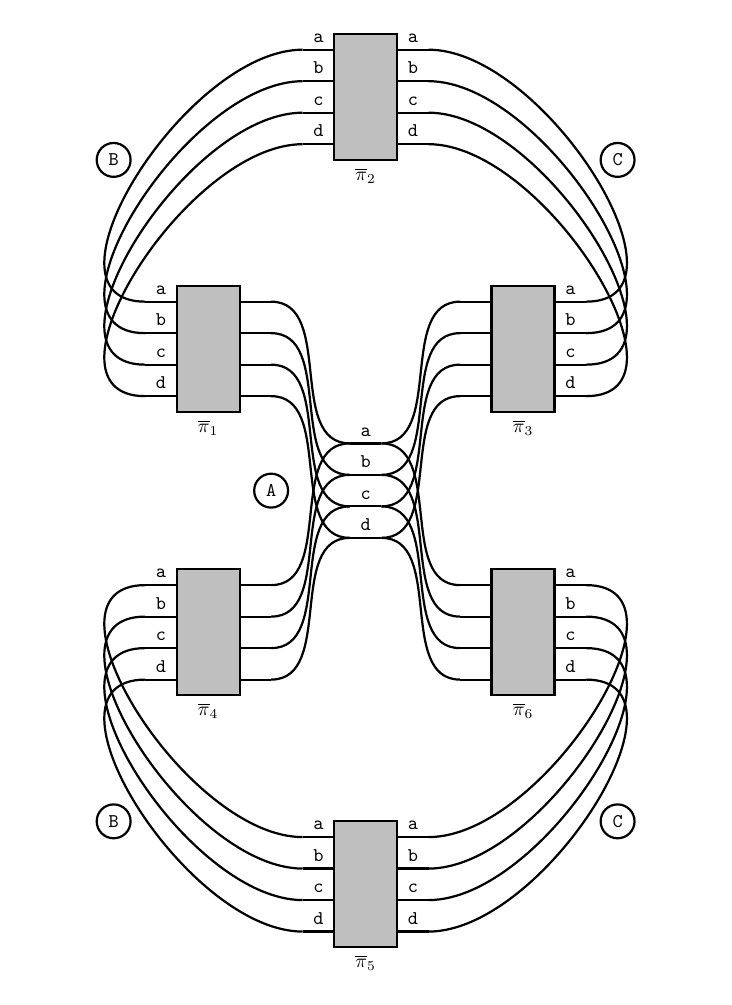
\begin{tikzpicture}[thick, scale=0.4, every node/.style={scale=0.7}]
				% Draw the box
				\draw[fill=lightgray] (0+5, 0+2) rectangle (2+5,4+2) node[midway] {};
				\node at (0+5+1, 0+2-0.5) {$\overline\pi_3$};

				% Draw the wires exiting the box
				\draw[-] (7, 5.5) -- (8,5.5) node[midway, above] {\texttt{a}};
				\draw[-] (7, 4.5) -- (8,4.5) node[midway, above] {\texttt{b}};
				\draw[-] (7, 3.5) -- (8, 3.5) node[midway, above] {\texttt{c}};
				\draw[-] (7,2.5) -- (8, 2.5) node[midway, above] {\texttt{d}};

				% Draw the wires entering the box
				\draw[-] (4, 5.5) -- (5,5.5) node[midway, above] {};
				\draw[-] (4, 4.5) -- (5,4.5) node[midway, above] {};
				\draw[-] (4, 3.5) -- (5, 3.5) node[midway, above] {};
				\draw[-] (4,2.5) -- (5, 2.5) node[midway, above] {};

				\draw[fill=lightgray] (0-5,0+2) rectangle (2-5,4+2) node[midway] {};
				\node at (0-5+1, 0+2-0.5) {$\overline\pi_1$};

				% Draw the wires entering the box
				\draw[-] (-13+7, 5.5) -- (-13+8,5.5) node[midway, above] {\texttt{a}};
				\draw[-] (-13+7, 4.5) -- (-13+8,4.5) node[midway, above] {\texttt{b}};
				\draw[-] (-13+7, 3.5) -- (-13+8, 3.5) node[midway, above] {\texttt{c}};
				\draw[-] (-13+7,2.5) -- (-13+8, 2.5) node[midway, above] {\texttt{d}};

				% Draw the wires exiting the box
				\draw[-] (-13+7+3, 5.5) -- (-13+8+3,5.5) node[midway, above] {};
				\draw[-] (-13+7+3, 4.5) -- (-13+8+3,4.5) node[midway, above] {};
				\draw[-] (-13+7+3, 3.5) -- (-13+8+3, 3.5) node[midway, above] {};
				\draw[-] (-13+7+3,2.5) -- (-13+8+3, 2.5) node[midway, above] {};

				\draw[fill=lightgray] (0,0+10) rectangle (2,4+10) node[midway] {};
				\node at (0+1, 0+10-0.5) {$\overline\pi_2$};

				% Draw the wires entering the box
				\draw[-] (-1, 3+10.5) -- (0, 3+10.5) node[midway, above] {\texttt{a}};
				\draw[-] (-1, 2+10.5) -- (0, 2+10.5) node[midway, above] {\texttt{b}};
				\draw[-] (-1, 1+10.5) -- (0, 1+10.5) node[midway, above] {\texttt{c}};
				\draw[-] (-1,0+10.5) -- (0,0+10.5) node[midway, above] {\texttt{d}};

				% Draw the wires exiting the box
				\draw[-] (3+-1, 3+10.5) -- (3+0, 3+10.5) node[midway, above]
				{\texttt{a}};
				\draw[-] (3+-1, 2+10.5) -- (3+0, 2+10.5) node[midway, above]
				{\texttt{b}};
				\draw[-] (3+-1, 1+10.5) -- (3+0, 1+10.5) node[midway, above]
				{\texttt{c}};
				\draw[-] (3+-1,0+10.5) -- (3+0,0+10.5) node[midway, above] {\texttt{d}};

				% Draw wires from 2 to 1
				\draw[-] (-6, 5.5) to[out=180, in=180] (-1, 13.5)
				node[midway, above] {};
				\draw[-] (-6, 4.5) to[out=180, in=180] (-1, 12.5)
				node[midway, above] {};
				\draw[-] (-6, 3.5) to[out=180, in=180] (-1, 11.5)
				node[midway, above] {};
				\draw[-] (-6, 2.5) to[out=180, in=180] (-1, 10.5)
				node[midway, above] {};

				% Draw wires from 3 to 2
				\draw[-] (8, 5.5) to[out=360, in=360] (3, 13.5) node[midway, above] {};
				\draw[-] (8, 4.5) to[out=360, in=360] (3, 12.5) node[midway, above] {};
				\draw[-] (8, 3.5) to[out=360, in=360] (3, 11.5) node[midway, above] {};
				\draw[-] (8, 2.5) to[out=360, in=360] (3, 10.5)
				node[midway, above] {};

				% Midway wires
				\draw[-] (0.5, 1) -- (1.5, 1) node[midway, above] {\texttt{a}};
				\draw[-] (0.5, 0) -- (1.5, 0) node[midway, above] {\texttt{b}};
				\draw[-] (0.5, -1) -- (1.5, -1) node[midway, above] {\texttt{c}};
				\draw[-] (0.5,-2) -- (1.5,-2) node[midway, above] {\texttt{d}};

				% Draw wires from 1 to midway
				\draw[-] (-2, 5.5) to[out=360, in=180] (0.5, 1) node[midway, above] {};
				\draw[-] (-2, 4.5) to[out=360, in=180] (0.5, 0) node[midway, above] {};
				\draw[-] (-2, 3.5) to[out=360, in=180] (0.5, -1) node[midway, above] {};
				\draw[-] (-2, 2.5) to[out=360, in=180] (0.5, -2) node[midway, above] {};

				% Draw wires from 2 to midway
				\draw[-] (4, 5.5) to[out=180, in=360] (1.5, 1) node[midway, above] {};
				\draw[-] (4, 4.5) to[out=180, in=360] (1.5, 0) node[midway, above] {};
				\draw[-] (4, 3.5) to[out=180, in=360] (1.5, -1) node[midway, above] {};
				\draw[-] (4, 2.5) to[out=180, in=360] (1.5, -2) node[midway, above] {};

				\draw[fill=lightgray] (0,0-15) rectangle (2,4-15) node[midway] {};
				\node at (0+1, 0+10-0.5-25) {$\overline\pi_5$};

				% Draw the wires entering the box
				\draw[-] (-1, 3+10.5-25) -- (0, 3+10.5-25) node[midway,
					above] {\texttt{a}};
				\draw[-] (-1, 2+10.5-25) -- (0, 2+10.5-25) node[midway,
					above] {\texttt{b}};
				\draw[-] (-1, 1+10.5-25) -- (0, 1+10.5-25) node[midway,
					above] {\texttt{c}};
				\draw[-] (-1,0+10.5-25) -- (0,0+10.5-25) node[midway, above]
				{\texttt{d}};

				% Draw the wires exiting the box
				\draw[-] (3+-1, 3+10.5-25) -- (3+0, 3+10.5-25) node[midway,
					above] {\texttt{a}};
				\draw[-] (3+-1, 2+10.5-25) -- (3+0, 2+10.5-25) node[midway,
					above] {\texttt{b}};
				\draw[-] (3+-1, 1+10.5-25) -- (3+0, 1+10.5-25) node[midway,
					above] {\texttt{c}};
				\draw[-] (3+-1,0+10.5-25) -- (3+0,0+10.5-25) node[midway,
					above] {\texttt{d}};

				\draw[fill=lightgray] (0-5,0+2-9) rectangle (2-5,4+2-9) node[midway] {};
				\node at (0-5+1, 0+2-0.5-9) {$\overline\pi_4$};

				% Draw the wires entering the box
				\draw[-] (-13+7, 5.5-9) -- (-13+8,5.5-9) node[midway, above]
				{\texttt{a}};
				\draw[-] (-13+7, 4.5-9) -- (-13+8,4.5-9) node[midway, above]
				{\texttt{b}};
				\draw[-] (-13+7, 3.5-9) -- (-13+8, 3.5-9) node[midway, above]
				{\texttt{c}};
				\draw[-] (-13+7,2.5-9) -- (-13+8, 2.5-9) node[midway, above]
				{\texttt{d}};

				% Draw the wires exiting the box
				\draw[-] (-13+7+3, 5.5-9) -- (-13+8+3,5.5-9) node[midway, above] {};
				\draw[-] (-13+7+3, 4.5-9) -- (-13+8+3,4.5-9) node[midway, above] {};
				\draw[-] (-13+7+3, 3.5-9) -- (-13+8+3, 3.5-9) node[midway, above] {};
				\draw[-] (-13+7+3,2.5-9) -- (-13+8+3, 2.5-9) node[midway, above] {};

				% Draw the box
				\draw[fill=lightgray] (0+5, 0+2-9) rectangle (2+5,4+2-9)
				node[midway] {};
				\node at (0+5+1, 0+2-0.5-9) {$\overline\pi_6$};

				% Draw the wires exiting the box
				\draw[-] (7, 5.5-9) -- (8,5.5-9) node[midway, above] {\texttt{a}};
				\draw[-] (7, 4.5-9) -- (8,4.5-9) node[midway, above] {\texttt{b}};
				\draw[-] (7, 3.5-9) -- (8, 3.5-9) node[midway, above] {\texttt{c}};
				\draw[-] (7,2.5-9) -- (8, 2.5-9) node[midway, above] {\texttt{d}};

				% Draw the wires entering the box
				\draw[-] (4, 5.5-9) -- (5,5.5-9) node[midway, above] {};
				\draw[-] (4, 4.5-9) -- (5,4.5-9) node[midway, above] {};
				\draw[-] (4, 3.5-9) -- (5, 3.5-9) node[midway, above] {};
				\draw[-] (4,2.5-9) -- (5, 2.5-9) node[midway, above] {};

				% Draw wires from 4 to 5
				\draw[-] (-6, 5.5-9) to[out=180, in=180] (-1, 13.5-25)
				node[midway, above] {};
				\draw[-] (-6, 4.5-9) to[out=180, in=180] (-1, 12.5-25)
				node[midway, above] {};
				\draw[-] (-6, 3.5-9) to[out=180, in=180] (-1, 11.5-25)
				node[midway, above] {};
				\draw[-] (-6, 2.5-9) to[out=180, in=180] (-1, 10.5-25)
				node[midway, above] {};

				% Draw wires from 5 to 6
				\draw[-] (8, 5.5-9) to[out=360, in=360] (3, 13.5-25)
				node[midway, above] {};
				\draw[-] (8, 4.5-9) to[out=360, in=360] (3, 12.5-25)
				node[midway, above] {};
				\draw[-] (8, 3.5-9) to[out=360, in=360] (3, 11.5-25)
				node[midway, above] {};
				\draw[-] (8, 2.5-9) to[out=360, in=360] (3, 10.5-25)
				node[midway, above] {};

				% Draw wires from 4 to midway
				\draw[-] (-2, 5.5-9) to[out=360, in=180] (0.5, 1)
				node[midway, above] {};
				\draw[-] (-2, 4.5-9) to[out=360, in=180] (0.5, 0)
				node[midway, above] {};
				\draw[-] (-2, 3.5-9) to[out=360, in=180] (0.5, -1)
				node[midway, above] {};
				\draw[-] (-2, 2.5-9) to[out=360, in=180] (0.5, -2)
				node[midway, above] {};

				% Draw wires from 2 to midway
				\draw[-] (4, 5.5-9) to[out=180, in=360] (1.5, 1) node[midway, above] {};
				\draw[-] (4, 4.5-9) to[out=180, in=360] (1.5, 0) node[midway, above] {};
				\draw[-] (4, 3.5-9) to[out=180, in=360] (1.5, -1)
				node[midway, above] {};
				\draw[-] (4, 2.5-9) to[out=180, in=360] (1.5, -2)
				node[midway, above] {};

				\node[draw,circle] at (-2, -0.5) {\texttt{A}};
				\node[draw,circle] at (-7, -11) {\texttt{B}};
				\node[draw,circle] at (-7, -11+21) {\texttt{B}};
				\node[draw,circle] at (-7+16, -11) {\texttt{C}};
				\node[draw,circle] at (-7+16, -11+21) {\texttt{C}};
			\end{tikzpicture}
		}
	\end{center}
	\caption{Multiple loops in the Bombe}
	\label{fig:multiloops}
\end{figure}
\noindent This increased electrical connections resulting in fewer
stops. We will return in the next chapter to the effect that multiple
loops has on the number of stops.

\subsection{Indicator Drums and Ring Setting}
The Bombe is set up with up to $12$ scramblers
\begin{center}
	$R_{x_1, y_1, z_1},\dots, R_{x_k, y_k, z_k}$
\end{center}
intended to encode the various positions of our Enigma machine while
enciphering our plaintext-ciphertext pairing. We assume that the
initial setting while encoding the message was \texttt{ZZZ}. It will
run through all $26^3$ positions of the Enigma machine until it finds
a stop. Suppose that at a stop the drums have positions
\begin{center}
	$R_{a_1, b_1, c_1},\dots, R_{a_k, b_k, c_k}$.
\end{center}
Given that our supposed ring setting was \texttt{ZZZ} (we will denote
(\texttt{26},
\texttt{26}, \texttt{26})), we now know that a candidate with a ring
setting of (\texttt{26},
\texttt{26}, \texttt{26}) and window setting of $(a_1, b_1, c_1)$
which should produce our expected plaintext at the location of the
first letter included in our loop. Of course, we want the plaintext
from the beginning of our plaintext-ciphertext pairing, so this
should actually occur at a window setting of
\begin{align}
	\label{eq:bombe_stop}
	(\texttt{Z} + (a_1-x_1)\text{ mod }26, \texttt{Z} + (b_1-y_1)\text{
		mod }26, \texttt{Z} + (c_1-z_1)\text{ mod }26)
\end{align}
with a ring setting of (\texttt{26},
\texttt{26}, \texttt{26}). Recall, that our assumed window setting at
the beginning of our plaintext-ciphertext pairing is \texttt{ZZZ}. We
want to move our window setting \ref{eq:bombe_stop} to correspond
with this but, in order to maintain permutation which produced the
stop, we must move the ring setting backwards by the same amount we
must move from \ref{eq:bombe_stop} to \texttt{ZZZ}. This displacement
is given by
\begin{align*}
	((a_1-x_1)\text{ mod }26, (b_1-y_1)\text{ mod }26, (c_1-z_1)\text{ mod }26)
\end{align*}
since the \texttt{Z}s cancel out. Then we must move our assumed ring
setting of (\texttt{26},
\texttt{26}, \texttt{26}) backwards by this same amount giving a ring setting of
\begin{align*}
	(\texttt{26} - (a_1-x_1)\text{ mod }26, \texttt{26} -
	(b_1-y_1)\text{ mod }26, \texttt{26} - (c_1-z_1)\text{ mod }26).
\end{align*}
Notice that $(a_1-x_1, b_1-y_1, c_1-z_1)$ is just the number of steps
our machine has made since it started. So, to get the ring position
corresponding to the start of our plaintext-ciphertext pairing we
just subtract the number of steps each rotor has made from our
assumed ring position (\texttt{26},\texttt{26}, \texttt{26}). Rather
than doing all this math, the Bombe was equipped with an additional
set of {\bf{indicator drums}} which began with labels \texttt{ZZZ}
and for each step the machine moved \emph{forward}, it moved the
indicator drum \emph{backward}. This means that when the machine
stopped, the indicator drums would immediately tell us the ring
setting which corresponded to our plaintext-ciphertext pairing. Then,
with this ring setting, setting our machine to the window setting
\texttt{ZZZ} would produce our expected plaintext-ciphertext
pairing\footnote{The actual rotors used in the Bombe scramblers were
	incorrect and did not match the true Enigma rotors by varying degrees
	of rotation depending on the rotor in question. This meant operators
	did not set their window settings to \texttt{ZZZ} but rather some
	small offset depending on which rotors were included. This meant if
	we used rotors (\texttt{II}, \texttt{V}, \texttt{III}) our window
	setting would be \texttt{YWY}}.

\subsection{Recovering the Plugboard}
Given a stop, we now know that for our hypothesized rotor order, a
window setting of \texttt{ZZZ}, and ring setting given by the
indicator drums we should be able to produce our plaintext-ciphertext
pair. However, we have yet to deduce the plugboard setting. The
genius of the Bombe is that much of the deduction required to workout
the plugboard setting has been done for us. Consider a possible stop
of the Bombe
\begin{center}
	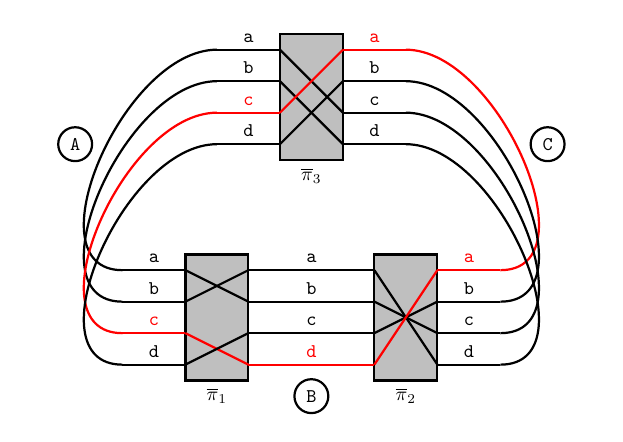
\begin{tikzpicture}[thick, scale=0.4, every node/.style={scale=0.7}]
		% Draw the box
		\draw[fill=lightgray] (2,-1.5) rectangle (4,2.5) node[midway] {};

		\node at (3, -2) {$\overline\pi_3$};

		% Draw the wires entering the box
		\draw[-] (0, 2) -- (2, 2) node[midway, above] {\texttt{a}};
		\draw[-] (0, 1) -- (2, 1) node[midway, above] {\texttt{b}};
		\draw[-, red] (0, 0) -- (2, 0) node[midway, above] {\texttt{c}};
		\draw[-] (0,-1) -- (2,-1) node[midway, above] {\texttt{d}};

		% Draw the wires exiting the box with crossed mappings
		\draw[-, red] (4, 2) -- (6,2) node[midway, above] {\texttt{a}};
		\draw[-] (4, 1) -- (6, 1) node[midway, above] {\texttt{b}};
		\draw[-] (4, 0) -- (6, 0) node[midway, above] {\texttt{c}};
		\draw[-] (4,-1) -- (6, -1) node[midway, above] {\texttt{d}};

		% Draw the lines inside the box to represent the mapping
		\draw[-] (2, 2) -- (4,0);
		\draw[-] (2, 1) -- (4, -1);
		\draw[-, red] (2, 0) -- (4, 2);
		\draw[-] (2,-1) -- (4, 1);

		\draw[-] (0-3, 2-7) to[out=180, in=180] (0, 2) node[midway, above] {};
		\draw[-] (0-3, 1-7) to[out=180, in=180] (0, 1) node[midway, above] {};
		\draw[-, red] (0-3, 0-7) to[out=180, in=180] (0, 0) node[midway, above] {};
		\draw[-] (0-3, -1-7) to[out=180, in=180] (0, -1)
		node[midway, above] {};

		\draw[- ,red] (6+3, 2-7) to[out=360, in=360] (6, 2) node[midway, above] {};
		\draw[-] (6+3, 1-7) to[out=360, in=360] (6, 1) node[midway, above] {};
		\draw[-] (6+3, 0-7) to[out=360, in=360] (6, 0) node[midway, above] {};
		\draw[-] (6+3, -1-7) to[out=360, in=360] (6, -1) node[midway, above] {};

		\draw[fill=lightgray] (2-3,-1.5-7) rectangle (4-3,2.5-7) node[midway] {};

		\node at (3-3, -2-7) {$\overline\pi_1$};

		% Draw the wires entering the box
		\draw[-] (0-3, 2-7) -- (2-3, 2-7) node[midway, above] {\texttt{a}};
		\draw[-] (0-3, 1-7) -- (2-3, 1-7) node[midway, above] {\texttt{b}};
		\draw[-, red] (0-3, 0-7) -- (2-3, 0-7) node[midway, above] {\texttt{c}};
		\draw[-] (0-3,-1-7) -- (2-3,-1-7) node[midway, above] {\texttt{d}};

		% Draw the wires exiting the box
		\draw[-] (4-3, 2-7) -- (6-3,2-7) node[right, above] {\texttt{a}};
		\draw[-] (4-3, 1-7) -- (6-3, 1-7) node[right, above] {\texttt{b}};
		\draw[-] (4-3, 0-7) -- (6-3, 0-7) node[right, above] {\texttt{c}};
		\draw[-, red] (4-3,-1-7) -- (6-3, -1-7) node[right, above] {\texttt{d}};

		% Draw the lines inside the box to represent the mapping
		\draw[-] (2-3, 2-7) -- (4-3, 1-7);
		\draw[-] (2-3, 1-7) -- (4-3, 2-7);
		\draw[-, red] (2-3, 0-7) -- (4-3, -1-7);
		\draw[-] (2-3,-1-7) -- (4-3, 0-7);

		\draw[fill=lightgray] (2+3,-1.5-7) rectangle (4+3,2.5-7) node[midway] {};

		\node at (3+3, -2-7) {$\overline\pi_2$};

		% Draw the wires entering the box
		\draw[-] (0+3, 2-7) -- (2+3, 2-7) node[midway, above] {};
		\draw[-] (0+3, 1-7) -- (2+3, 1-7) node[midway, above] {};
		\draw[-] (0+3, 0-7) -- (2+3, 0-7) node[midway, above] {};
		\draw[-, red] (0+3,-1-7) -- (2+3,-1-7) node[midway, above] {};

		% Draw the wires exiting the box
		\draw[-, red] (4+3, 2-7) -- (6+3,2-7) node[midway, above] {\texttt{a}};
		\draw[-] (4+3, 1-7) -- (6+3, 1-7) node[midway, above] {\texttt{b}};
		\draw[-] (4+3, 0-7) -- (6+3, 0-7) node[midway, above] {\texttt{c}};
		\draw[-] (4+3,-1-7) -- (6+3, -1-7) node[midway, above] {\texttt{d}};

		\draw[-] (2+3, 2-7) -- (4+3, -1-7);
		\draw[-] (2+3, 1-7) -- (4+3, 0-7);
		\draw[-] (2+3, 0-7) -- (4+3, 1-7);
		\draw[-, red] (2+3,-1-7) -- (4+3, 2-7);

		\node[draw,circle] at (-4.5, -1) {\texttt{A}};
		\node[draw,circle] at (3, -9) {\texttt{B}};
		\node[draw,circle] at (10.5, -1) {\texttt{C}};

	\end{tikzpicture}
\end{center}
Our hypothesized plugboard setting was that \texttt{A} was steckered
to \texttt{C} and we found no logical contradictions thus producing a
stop. This means that at a minimum we recover that $S(\texttt{A}) =
	\texttt{C}$. However, we may as well have hypothesis that \texttt{B}
was steckered to \texttt{D} and thus we would have applied current to
wire \texttt{Bd}. Note that this wire is included in our connected
component so we would have recovered the exact same stop. That is,
the statement $S(\texttt{B}) = \texttt{D}$ also produced no logical
contradictions. Similarly, reading off cable \texttt{C} we would
recover $S(\texttt{C}) = \texttt{A}$ though we already knew this from
our first hypothesis. Thus, for each cable in our loop we recover a
plugboard setting consistent with our initial hypothesis (though some
of these may be redundant). For a sufficiently long loop we can
recover several plugboard setting just by seeing which wires are
electrified on which cables.
\subsubsection{Checking Machines}
While looking at the internal wiring will, in fact, derive such
plugboard settings, from an operator's perspective the Bombe only
displayed which steckering our cable involved in our initial
hypothesis produced. For this reason, a special device was produced
called a {\bf{checking machine}} whose sole purpose was to derive
these plugboard settings from a stop of the Bombe. We will consider
one such derivation.
% Wren reference https://wrens.org.uk/second-world-war-codebreaker/ %
\\\\The checking machine was effectively an Enigma machine with no
plugboard attachment and no rotor advancement mechanism --
effectively, the checking machine represents a fixed
$\overline\sigma_i$. Suppose the operator (known as a
	{\bf{wren}})\footnote{Wren comes from the abbreviation WRN of the
	Women's Royal Navy Service. Such members became the primary operators
	of Bombes at Bletchley Park.} knew from the Bombe stop that our
hypothesis letter \texttt{A} was steckered to \texttt{C} (i.e.
$S(\texttt{A} = \texttt{C}$)). Further, from our loop the wren might know that
\[
	\sigma_1(\texttt{A}) = \texttt{B}
\]
We then have that
\begin{align*}
	S(\texttt{B}) & = S(\sigma_1(\texttt{A}))                \\
	              & = SS^{-1}\overline\sigma_1 S(\texttt{A}) \\
	              & = \overline\sigma_1(\texttt{D})
\end{align*}
Then to determine what letter is steckered to \texttt{B}, the wren
only needs to set their ring settings to that given by the indicator,
the window settings to that corresponding to $\sigma_1$, and input
\texttt{D}. Now using this newly deduced steckering the wren can
produce the steckering of the next letter in the loop until we have
deduced the steckerings corresponding to each letter in our loop.

\subsubsection{Invalid Stops}
If at this stage we find that a deduced plugboard setting contradicts
an earlier plugboard setting we discovered, this means that the point
at which the Bombe stopped is incorrect! Recall that the Bombe stops
when there are no logical contradictions gleamed from its setup and
the information in the loop -- this does not mean no logical
contradictions exist. Further, even if no logical contradictions
existed that does not mean this is the only such setting which would
be logically consistent with our plaintext (though this is certainly
less likely). The use of the Bombe is thus a trial-and-error
procedure. We run the machine until we find a candidate stop, then we
check for possible further logical contradictions, and if such
contradictions are found we continue from where we left off. Many
additions we discuss later in this chapter are designed with the sole
purpose of reducing the number of stops we need to check down to a
tractable number.
\\\\If we find our stop has valid plugboard settings, we can recover
any remaining settings is quite easily. We can attempt to decrypt our
ciphertext with our window setting of \texttt{ZZZ}, our ring setting
given by the indicator drums, and our plguboard settings we
discovered from the stop. If we find that there are letters which do
not match our expected plaintext we can deduce what plugboard
settings need to be added to switch out incorrect letters with their
correct plaintext letters. In this way we can recover the entirety of
the plugboard settings.
\subsection{Recovering the Ring Settings}
By this point we know that for our hypothesized rotor ordering, a
window setting of \texttt{ZZZ}, a ring setting given by the indicator
drums, and a plugboard setting deduced from the state of the stop as
well as additional logical induction, we can produce the desired
ciphertext-plaintext pairing. However, this does not mean the ring
setting that we have is the true ring setting. We assumed that
turnover did not occur during our crib so in this case we can adjust
our window setting and ring setting arbitrarily (so long as we keep
their relative distances the same). Of course, eventually turnover
will occur, at which point the discrepancy between our ring setting
and the true ring setting will become apparent.
\\\\We will first illustrate how to recover the true ring setting of
the rightmost rotor. We begin by setting our Enigma as previously
described and inputting the ciphertext. This should produce our
expected plaintext. As we keep inputting ciphertext beyond our known
plaintext we will recover additional plaintext in the message.
Eventually, turnover will occur and we will begin deciphering
gibberish since our ring setting is not the true ring setting. To
account for this, we can move our ring setting forward by one step
(which means we must also move our window setting forward by one to
maintain our permutation) and we can perform the same procedure,
investigating if we get gibberish. Eventually, we will have arrived
at the true ring setting and our deciphering will begin producing
additional plaintext.
\\\\To recover the ring setting of the other two rotors we employ the
same procedure though it requires a great deal of ciphertext as
turnover becomes less and less frequent as we consider the middle and
leftmost rotor respectively.

\subsection{Recovering the Rotor Order}
In its full form the Bombe was constructed with $3$ rows each
equipped with 12 scramblers. For a single plaintext-ciphertext
pairing we could test multiple rotor orders simultaneously. If our
plaintext-ciphertext pairing is shorter than $12$ characters we could
test $3$ rotor orders concurrently. If it is longer then we may need
to split it into two separate pairings spread across multiple rows
meaning that we may only test $1$ or $2$ rotor orders. Further, over
the course of the war many Bombes were produced. This meant that it
was feasible to test all $60$ rotor orderings against our
plaintext-ciphertext pairing to see which orderings generated valid
stops, thus allowing us to deduce the correct rotor order. In doing
this, we have now managed to recover all of the relevant settings of
the daily key.

\subsection{Turnover}
Recall that when we initially set up our Bombe, we set each scrambler
to correspond to a location in our plaintext -- the first location
being $\texttt{ZZZ}$, the second being \texttt{ZZA}, and so on. As
mentioned previously, the assumption that only the righthand rotor
advanced in our window setting while enciphering the plaintext is
only true if no turnover occurs. If turnover occured during the
message encipherment, our machine will not produce correct stops.
\\\\To account for this we will split up our message into multiple
parts. Consider a plaintext-ciphertext pairing that is $26$
characters long. We are guaranteed to have a turnover of the middle
rotor during the encipherment of this message. However, we know that
the turnover must have occured in either the first half or the second
half of the message. Thus, one half of the message assuredly had no
turnover during its encipherment. This means that if we split our
message into two $13$ character plaintext-ciphertext pairings, at
least one of these will produce valid stops which will ultimately
guide us to our daily key. In general, as long as our message is
shorter than $26$ characters we can split the message into components
such that one component is guaranteed to not have turnover. If the
message is longer than $26$ characters there could be $2$ or more
turnovers during encipherment meaning that splitting the text in this
way would no longer guarantee valid stops but, as we will see in our
analysis in the next chapter, a plaintext-ciphertext pairing of
length $26$ is more than sufficient to produce a small number of
stops so this does not present an issue.
\subsection{Cribs and Menus}

% \begin{chapquote}{Gordon Welchman, \textit{The Hut Six Story Page 120}}
%   The bombes were useless without a crib. If a crib could be found by
%   the Hut 6 watch, the task of the bombe was simply to reduce the
%   assumptions of wheel order and scrambler positions that required
%   ``further analysis'' to a managable number.
% \end{chapquote}
We began with the supposition that the
cryptographer is given a known plaintext-ciphertext pairing. Unless
the cryptographer was able to intercept
a set of communications before and after encryption this supposition
seems unrealistic. However, cryptanalysts at Bletchley park
employed two clever tricks that allowed for such pairings to be
deduced with reasonable effectiveness. First, analysts were able to
cross-reference known information to theorize likely phrases in a
message. For instance, if the weather on a particular day was windy
with a chance of rain, we would expect that the weather report (which
intellegence knew arrived from specific channels at specific times)
would likely contain phrases like ``weather'', ``wind'', or ``rain''.
The second trick used by analysts was the use of permutation theory to
eliminate locations in the ciphertext where the plaintext could not
feasibly have been enciphered.
% http://www.ellsbury.com/bombe1.htm %
\\\\Recall that one consequence of the Enigma machine being a
conjugate of the reflector is that no letter can be enciphered to
itself. On D-Day the weather report had the following ciphertext
\begin{center}
	\texttt{QFZWRWIVTYRESXBFOGKUHQBAISEZ}
\end{center}
Given that this was a report the weather in the Bay of Biscay, we
suspect it to contain the following plaintext
\begin{center}
	\texttt{WETTERVORHERSAGEBISKAYA}
\end{center}
If we overlay our ciphertext on top of our plaintext as follows
\begin{align*}
	 & \texttt{QFZWRWIVTYRE}{\uline{\texttt{S}}}\texttt{XBFOGKUHQBAISEZ} \\
	 & \texttt{WETTERVORHER}{\uline{\texttt{S}}}\texttt{AGEBISKAYA.....}
\end{align*}
we notice that at the 13th position, the letter \texttt{S} appears in
both the plaintext and the ciphertext. We know that such an
encipherment is impossible and therefore the suspected plaintext
cannot begin at this location. If we slide the plaintext along our
ciphertext we get the following
\begin{align*}
	 & \texttt{QFZWRWIVTYRESXBFOGKUHQBAISEZ}
	\\
	 & \texttt{WETTERVORHER}{\uline{\texttt{S}}}\texttt{AGEBISKAYA.....}
	\\
	 &
	\texttt{.WETTER}{\uline{\texttt{V}}}\texttt{ORH}{\uline{\texttt{E}}}\texttt{RSAGEBISKAY}{\uline{\texttt{A}}}\texttt{....}
	\\
	 & \texttt{..WETTE}{\uline{\texttt{R}}}\texttt{VORHERSAGEBISKAYA...}
	\\
	 &
	\texttt{...}{\uline{\texttt{W}}}\texttt{ETTERVORHERSA}{\uline{\texttt{G}}}\texttt{EBISK}{\uline{\texttt{A}}}\texttt{YA...}
	\\
	 & \texttt{....WETTERVORHERSAGEBISKAYA..}
	\\
\end{align*}
We can see that at offsets $0-3$ we have coincidences between the
plaintext and the ciphertext that would make enciphering at this
position impossible. Only at an offset of $4$ do we observe no
coincidences. Such a potentially valid location for enciphering is
known as a {\bf{crib}}. We may find many such cribs for a given
transmission and suspected plaintext, but if our suspected plaintext
is long the likelihood of this occurring goes down significantly so
we expect to find only a few cribs.
\\\\Now equipped with our crib
\begin{figure}[H]
	\begin{center}
		\texttt{RWIVTYRESXBFOGKUHQBAISE}  \\
		\texttt{WETTERVORHERSAGEBISKAYA} \\
	\end{center}
	\caption{Example crib}
	\label{fig:crib}
\end{figure}
\noindent We can generate a diagramatic representation of our
plaintext-ciphertext pairing called a {\bf{menu}} which will be used
to wire up our Bombe. We assume the enciphering starts with window
setting \texttt{ZZZ} so we will denote which window setting takes
each letter to the next.
\begin{figure}[H]
	\begin{center}
		\scalebox{0.8}{
			\begin{tikzpicture}[>=stealth, every node/.style={}]
				% Manual node positions
				\node (E) at (0,0) {\texttt{E}};
				\node (O) at (3,1.5) {\texttt{0}};
				\node (B) at (0,3) {\texttt{B}};
				\node (U) at (-3,3) {\texttt{U}};
				\node (S) at (6,3) {\texttt{S}};
				\node (Y) at (9,3) {\texttt{Y}};
				\node (G) at (-6,3) {\texttt{G}};
				\node (H) at (0,6) {\texttt{H}};
				\node (X) at (-3,6) {\texttt{X}};
				\node (W) at (3,0) {\texttt{W}};
				\node (R) at (6,0) {\texttt{R}};
				\node (F) at (9,0) {\texttt{F}};
				\node (A) at (-3,0) {\texttt{A}};
				\node (I) at (-3,-3) {\texttt{I}};
				\node (Q) at (-6,-3) {\texttt{Q}};
				\node (T) at (0,-3) {\texttt{T}};
				\node (K) at (-6,0) {\texttt{K}};
				\node (V) at (6,-3) {\texttt{V}};

				% Connections
				\draw[-] (E) -- (W) node[midway, above, sloped] {\texttt{ZZB}};
				\draw[-] (W) -- (R) node[midway, above, sloped] {\texttt{ZZA}};
				\draw[-] (R) -- (F) node[midway, above, sloped] {\texttt{ZZL}};
				\draw[-] (R) -- (Y) node[midway, above, sloped] {\texttt{ZZF}};
				\draw[-] (E) -- (O) node[midway, above, sloped] {\texttt{ZZH}};
				\draw[-] (O) -- (S) node[midway, above, sloped] {\texttt{ZZM}};
				\draw[-] (S) -- (Y) node[midway, above, sloped] {\texttt{ZZV}};
				\draw[-] (R) -- (S) node[midway, above, sloped] {\texttt{ZZI}};
				\draw[-] (B) -- (S) node[midway, above, sloped] {\texttt{ZZS}};
				\draw[-] (E) -- (B) node[midway, above, sloped] {\texttt{ZZK}};
				\draw[-] (B) -- (H) node[midway, above, sloped] {\texttt{ZZQ}};
				\draw[-] (X) -- (H) node[midway, above, sloped] {\texttt{ZZJ}};
				\draw[-] (U) -- (E) node[midway, above, sloped] {\texttt{ZZP}};
				\draw[-] (G) -- (A) node[midway, above, sloped] {\texttt{ZZN}};
				\draw[-] (A) -- (E) node[midway, above, sloped] {\texttt{ZZW}};
				\draw[-] (K) -- (G) node[midway, above, sloped] {\texttt{ZZO}};
				\draw[-] (K) -- (A) node[midway, above, sloped] {\texttt{ZZT}};
				\draw[-] (T) -- (E) node[midway, above, sloped] {\texttt{ZZE}};
				\draw[-] (I) -- (A) node[midway, above, sloped] {\texttt{ZZU}};
				\draw[-] (Q) -- (I) node[midway, above, sloped] {\texttt{ZZR}};
				\draw[-] (I) -- (T) node[midway, above, sloped] {\texttt{ZZC}};
				\draw[-] (T) -- (V) node[midway, above, sloped] {\texttt{ZZD}};
				\draw[-] (V) -- (R) node[midway, above, sloped] {\texttt{ZZG}};

			\end{tikzpicture}}
	\end{center}
	\caption{Example menu}
	\label{fig:menu}
\end{figure}
\noindent Upon looking at this menu one might ask the question of why
we include connections like the one between \texttt{X} and \texttt{H}
if they are not included in any loop? From our earlier machine
description its clear that such connection will never electrify
additional wires. That is, they will only permute the incoming
electrified wires but never increasing the quantity of electrified
wires since there is no feedback. Thus they add no additional value
save for perhaps slightly more plugboard information. However, an
addition to the machine made by Gordon Welchman made use of such
connections and produced more electrified wires even within the loops
themselves, thus reducing the total number of stops needing to be checked.
% the Eniga machine is
% a series of 13 disjoint transpositions. Mathematically, this is
% because at each stage the permutation formed by the machine is just a
% conjugate of the reflector which has a $2^{13}$ cycle-type.
% \\\\ location of \emph{cribs} -- locations in the enciphered text
% that could plausibly have been generated from the suspsected
% plaintext phrases.

\subsection{Diagonal Board}
Recall that a wire \texttt{Xy} becoming electrified is consistent
with the deduction that $S(\texttt{X}) = \texttt{Y}$. But this
deduction is equivalent to the statement $S(\texttt{Y}) =
	\texttt{X}$. It follows then that if we apply current to \texttt{Yx}
this will be entirely consistent with our current deductions and thus
there will be no new logical contradictions introduced by this
additional current. That is, for any wire \texttt{Xy} we can connect
it directly to \texttt{Yx} through what was called a {\bf{diagonal
			board}}. In our diagram this can be viewed as follows
\begin{figure}[H]
	\begin{center}
		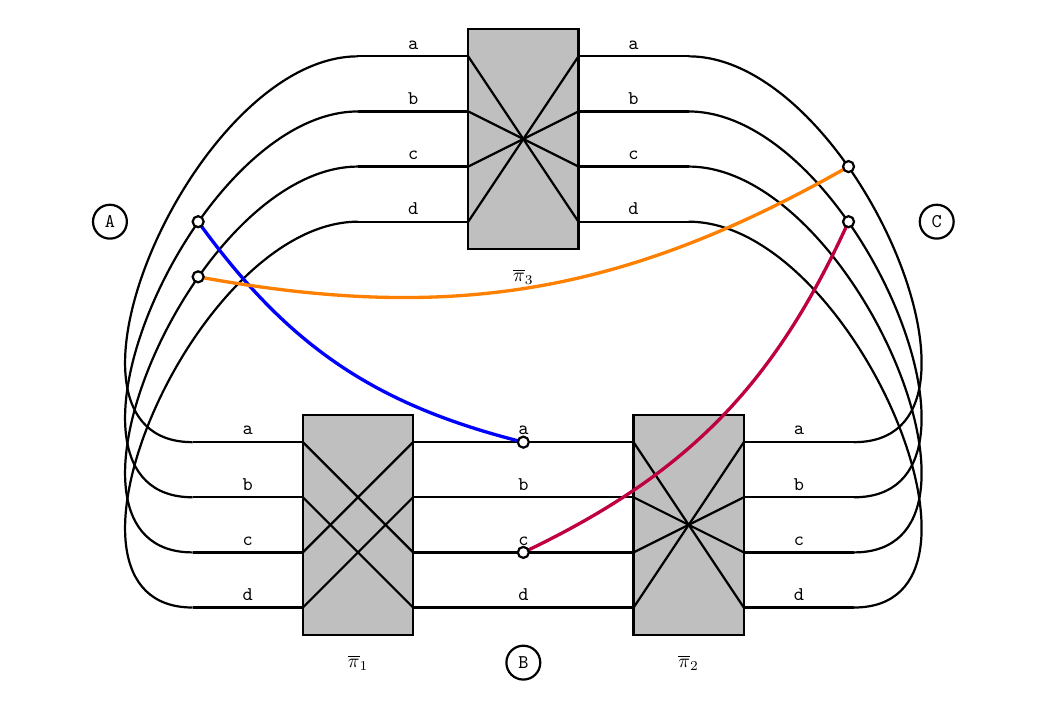
\begin{tikzpicture}[thick, scale=0.7, every node/.style={scale=0.7}]
			% Draw the box
			\draw[fill=lightgray] (2,-1.5) rectangle (4,2.5) node[midway] {};

			\node at (3, -2) {$\overline\pi_3$};

			% Draw the wires entering the box
			\draw[-] (0, 2) -- (2, 2) node[midway, above] {\texttt{a}};
			\draw[-] (0, 1) -- (2, 1) node[midway, above] {\texttt{b}};
			\draw[-] (0, 0) -- (2, 0) node[midway, above] {\texttt{c}};
			\draw[-] (0,-1) -- (2,-1) node[midway, above] {\texttt{d}};

			% Draw the wires exiting the box with crossed mappings
			\draw[-] (4, 2) -- (6,2) node[midway, above] {\texttt{a}};
			\draw[-] (4, 1) -- (6, 1) node[midway, above] {\texttt{b}};
			\draw[-] (4, 0) -- (6, 0) node[midway, above] {\texttt{c}};
			\draw[-] (4,-1) -- (6, -1) node[midway, above] {\texttt{d}};

			% Draw the lines inside the box to represent the mapping
			\draw[-] (2, 2) -- (4, -1);
			\draw[-] (2, 1) -- (4, 0);
			\draw[-] (2, 0) -- (4, 1);
			\draw[-] (2,-1) -- (4, 2);

			\draw[-] (0-3, 2-7) to[out=180, in=180] (0, 2) node[midway, above] {};
			\draw[-] (0-3, 1-7) to[out=180, in=180] (0, 1) node[midway, above] {};
			\draw[-] (0-3, 0-7) to[out=180, in=180] (0, 0) node[midway, above] {};
			\draw[-] (0-3, -1-7) to[out=180, in=180] (0, -1)
			node[midway, above] {};

			\draw[-] (6+3, 2-7) to[out=360, in=360] (6, 2) node[midway, above] {};
			\draw[-] (6+3, 1-7) to[out=360, in=360] (6, 1) node[midway, above] {};
			\draw[-] (6+3, 0-7) to[out=360, in=360] (6, 0) node[midway, above] {};
			\draw[-] (6+3, -1-7) to[out=360, in=360] (6, -1) node[midway, above] {};

			\draw[fill=lightgray] (2-3,-1.5-7) rectangle (4-3,2.5-7) node[midway] {};

			\node at (3-3, -2-7) {$\overline\pi_1$};

			% Draw the wires entering the box
			\draw[-] (0-3, 2-7) -- (2-3, 2-7) node[midway, above] {\texttt{a}};
			\draw[-] (0-3, 1-7) -- (2-3, 1-7) node[midway, above] {\texttt{b}};
			\draw[-] (0-3, 0-7) -- (2-3, 0-7) node[midway, above] {\texttt{c}};
			\draw[-] (0-3,-1-7) -- (2-3,-1-7) node[midway, above] {\texttt{d}};

			% Draw the wires exiting the box
			\draw[-] (4-3, 2-7) -- (6-3,2-7) node[right, above] {\texttt{a}};
			\draw[-] (4-3, 1-7) -- (6-3, 1-7) node[right, above] {\texttt{b}};
			\draw[-] (4-3, 0-7) -- (6-3, 0-7) node[right, above] {\texttt{c}};
			\draw[-] (4-3,-1-7) -- (6-3, -1-7) node[right, above] {\texttt{d}};

			% Draw the lines inside the box to represent the mapping
			\draw[-] (2-3, 2-7) -- (4-3, 0-7);
			\draw[-] (2-3, 1-7) -- (4-3, -1-7);
			\draw[-] (2-3, 0-7) -- (4-3, 2-7);
			\draw[-] (2-3,-1-7) -- (4-3, 1-7);

			\draw[fill=lightgray] (2+3,-1.5-7) rectangle (4+3,2.5-7) node[midway] {};

			\node at (3+3, -2-7) {$\overline\pi_2$};

			% Draw the wires entering the box
			\draw[-] (0+3, 2-7) -- (2+3, 2-7) node[midway, above] {};
			\draw[-] (0+3, 1-7) -- (2+3, 1-7) node[midway, above] {};
			\draw[-] (0+3, 0-7) -- (2+3, 0-7) node[midway, above] {};
			\draw[-] (0+3,-1-7) -- (2+3,-1-7) node[midway, above] {};

			% Draw the wires exiting the box
			\draw[-] (4+3, 2-7) -- (6+3,2-7) node[midway, above] {\texttt{a}};
			\draw[-] (4+3, 1-7) -- (6+3, 1-7) node[midway, above] {\texttt{b}};
			\draw[-] (4+3, 0-7) -- (6+3, 0-7) node[midway, above] {\texttt{c}};
			\draw[-] (4+3,-1-7) -- (6+3, -1-7) node[midway, above] {\texttt{d}};

			\draw[-] (2+3, 2-7) -- (4+3, -1-7);
			\draw[-] (2+3, 1-7) -- (4+3, 0-7);
			\draw[-] (2+3, 0-7) -- (4+3, 1-7);
			\draw[-] (2+3,-1-7) -- (4+3, 2-7);

			\node[draw,circle] at (-4.5, -1) {\texttt{A}};
			\node[draw,circle] at (3, -9) {\texttt{B}};
			\node[draw,circle] at (10.5, -1) {\texttt{C}};

			% Diagonal wires
			\draw[-, blue, very thick] (3,2-7) to[bend left=20] (-3+0.1, 2-3);
			\draw[fill=white] (-3+0.1, 2-3) circle (0.1);
			\draw[fill=white] (3, 2-7) circle (0.1);

			\draw[-, orange,  very thick] (9-0.1,2-2) to[bend left=20] (-3+0.1, 2-4);
			\draw[fill=white] (9-0.1, 2-2) circle (0.1);
			\draw[fill=white] (-3+0.1, 2-4) circle (0.1);

			\draw[-, purple, very thick] (3,0-7) to[bend right=20] (9-0.1, 2-3);
			\draw[fill=white] (3, 0-7) circle (0.1);
			\draw[fill=white] (9-0.1, 2-3) circle (0.1);

		\end{tikzpicture}
	\end{center}
	\caption{Diagonal wires}
	\label{fig:diagonal}
\end{figure}
\noindent This significantly increases the number of connections,
adding $\frac{k(k-1)}{2}$ new wires where $k$ is the number of
scramblers in the loop. Adding more connections increases electrical
connectivity thus reducing the number of stops. In fact, prior to the
use of the diagonal board, often $3$ loops needed to be present in
the crib to have a tractable number of stops. With the addition of
the diagonal board this could be significantly reduced and made the
use of the Bombe practical.
\\\\For instance, in our example from figure~\ref{fig:diagonal},
without the diagonal such a state would produce a stop with
hypothesis $S(\texttt{A}) = \texttt{D}$. However, adding the diagonal
wires would cause all wires to have current flowing through them --
meaning that our original stop must have been a false one, only
revealed by the addition of new, consistent deductions which ruled
out all possible plugboard settings.
\\\\This also meant that connections in our menu not included in a
loop, such as the connection in \ref{fig:menu} between \texttt{X} and
\texttt{H}, could now produce feedback within our loops through the
diagonal board connections. This made such connections valuable
additions to a menu.
\subsection{The Machine Gun}
Even with the Bombe and the diagonal board we still have more
deductions that can be made to rule out certain settings. Consider
our first stop we examined from figure~\ref{fig:correct_stecker}.
\begin{center}
	\begin{minipage}{0.45\textwidth}
		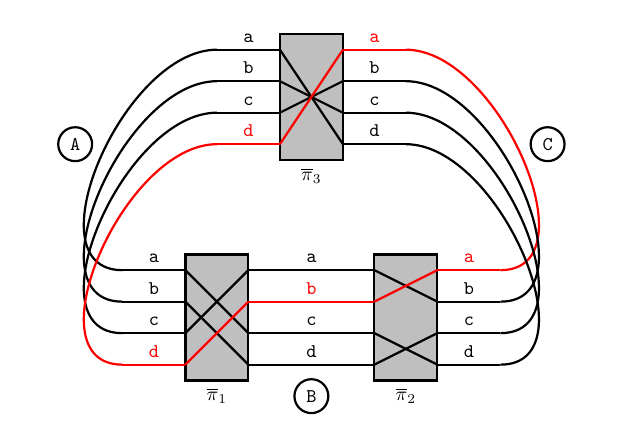
\begin{tikzpicture}[thick, scale=0.4, every node/.style={scale=0.7}]
			% Draw the box
			\draw[fill=lightgray] (2,-1.5) rectangle (4,2.5) node[midway] {};

			\node at (3, -2) {$\overline\pi_3$};

			% Draw the wires entering the box
			\draw[-] (0, 2) -- (2, 2) node[midway, above] {\texttt{a}};
			\draw[-] (0, 1) -- (2, 1) node[midway, above] {\texttt{b}};
			\draw[-] (0, 0) -- (2, 0) node[midway, above] {\texttt{c}};
			\draw[-, red] (0,-1) -- (2,-1) node[midway, above] {\texttt{d}};

			% Draw the wires exiting the box with crossed mappings
			\draw[-, red] (4, 2) -- (6,2) node[midway, above] {\texttt{a}};
			\draw[-] (4, 1) -- (6, 1) node[midway, above] {\texttt{b}};
			\draw[-] (4, 0) -- (6, 0) node[midway, above] {\texttt{c}};
			\draw[-] (4,-1) -- (6, -1) node[midway, above] {\texttt{d}};

			% Draw the lines inside the box to represent the mapping
			\draw[-] (2, 2) -- (4,-1);
			\draw[-] (2, 1) -- (4, 0);
			\draw[-] (2, 0) -- (4, 1);
			\draw[-, red] (2,-1) -- (4, 2);

			\draw[-] (0-3, 2-7) to[out=180, in=180] (0, 2) node[midway, above] {};
			\draw[-] (0-3, 1-7) to[out=180, in=180] (0, 1) node[midway, above] {};
			\draw[-] (0-3, 0-7) to[out=180, in=180] (0, 0) node[midway, above] {};
			\draw[-, red] (0-3, -1-7) to[out=180, in=180] (0, -1)
			node[midway, above] {};

			\draw[- ,red] (6+3, 2-7) to[out=360, in=360] (6, 2)
			node[midway, above] {};
			\draw[-] (6+3, 1-7) to[out=360, in=360] (6, 1) node[midway, above] {};
			\draw[-] (6+3, 0-7) to[out=360, in=360] (6, 0) node[midway, above] {};
			\draw[-] (6+3, -1-7) to[out=360, in=360] (6, -1) node[midway, above] {};

			\draw[fill=lightgray] (2-3,-1.5-7) rectangle (4-3,2.5-7) node[midway] {};

			\node at (3-3, -2-7) {$\overline\pi_1$};

			% Draw the wires entering the box
			\draw[-] (0-3, 2-7) -- (2-3, 2-7) node[midway, above] {\texttt{a}};
			\draw[-] (0-3, 1-7) -- (2-3, 1-7) node[midway, above] {\texttt{b}};
			\draw[-] (0-3, 0-7) -- (2-3, 0-7) node[midway, above] {\texttt{c}};
			\draw[-, red] (0-3,-1-7) -- (2-3,-1-7) node[midway, above] {\texttt{d}};

			% Draw the wires exiting the box
			\draw[-] (4-3, 2-7) -- (6-3,2-7) node[right, above] {\texttt{a}};
			\draw[-, red] (4-3, 1-7) -- (6-3, 1-7) node[right, above] {\texttt{b}};
			\draw[-] (4-3, 0-7) -- (6-3, 0-7) node[right, above] {\texttt{c}};
			\draw[-] (4-3,-1-7) -- (6-3, -1-7) node[right, above] {\texttt{d}};

			% Draw the lines inside the box to represent the mapping
			\draw[-] (2-3, 2-7) -- (4-3, 0-7);
			\draw[-] (2-3, 1-7) -- (4-3, -1-7);
			\draw[-] (2-3, 0-7) -- (4-3, 2-7);
			\draw[-, red] (2-3,-1-7) -- (4-3, 1-7);

			\draw[fill=lightgray] (2+3,-1.5-7) rectangle (4+3,2.5-7) node[midway] {};

			\node at (3+3, -2-7) {$\overline\pi_2$};

			% Draw the wires entering the box
			\draw[-] (0+3, 2-7) -- (2+3, 2-7) node[midway, above] {};
			\draw[-, red] (0+3, 1-7) -- (2+3, 1-7) node[midway, above] {};
			\draw[-] (0+3, 0-7) -- (2+3, 0-7) node[midway, above] {};
			\draw[-] (0+3,-1-7) -- (2+3,-1-7) node[midway, above] {};

			% Draw the wires exiting the box
			\draw[-, red] (4+3, 2-7) -- (6+3,2-7) node[midway, above] {\texttt{a}};
			\draw[-] (4+3, 1-7) -- (6+3, 1-7) node[midway, above] {\texttt{b}};
			\draw[-] (4+3, 0-7) -- (6+3, 0-7) node[midway, above] {\texttt{c}};
			\draw[-] (4+3,-1-7) -- (6+3, -1-7) node[midway, above] {\texttt{d}};

			\draw[-] (2+3, 2-7) -- (4+3, 1-7);
			\draw[-, red] (2+3, 1-7) -- (4+3, 2-7);
			\draw[-] (2+3, 0-7) -- (4+3, -1-7);
			\draw[-] (2+3,-1-7) -- (4+3, 0-7);

			\node[draw,circle] at (-4.5, -1) {\texttt{A}};
			\node[draw,circle] at (3, -9) {\texttt{B}};
			\node[draw,circle] at (10.5, -1) {\texttt{C}};

		\end{tikzpicture}
	\end{minipage}
\end{center}
This stop may seem to imply we found no logical inconsitencies in our
deductions stemming from the hypothesis that $S(\texttt{A}) =
	\texttt{D}$. However, when a wren goes to check the settings found,
they will discover that this setting produces a contradictory
plugboard setting of $S(\texttt{A}) = \texttt{C}$ -- thus ruling out
this stop. Is there a means by which we could have detected this
without having to manually work it out on a checking machine?
\\\\Recall that before we introduced the checking machine, we noted
that the plugboard settings we would deduce from the checking machine
were implictly encoded in the internal state of the wires of the
machine. In particular since wire $\texttt{Ca}$ was active, we could
have immediately deduced that $S(\texttt{A})= \texttt{C}$ without
having to employ a checking machine. However, these wires states are
not easy for a human to read and would require complex manual
analysis of the underlying cables. Instead, a device called the
	{\bf{machine gun}} was developed which examined the state of the
diagonal board at a given stop to determine if logical contradictions
were present among the deduced plugboard settings. When a stop
occured, the machine gun would be brought in. The device then used a
series of uniselectors to quickly switch through the diagonal board
contacts to search for a pair of deduced steckerings that had a
common letter (thus producing a logical contradiction). The machine
got its name from the sudden loud burst of sound produced when the
uniselectors ran through the diagonal board.
\\\\Even with such a device many stops still needed to be checked by
the wrens since the machine gun only detected logical inconsistencies
in regards to plugboard setting overlap and thus still produced false stops.

\section{Banburismus}
Early in this chapter we discussed the changes made to the Enigma
protocol that necessitated the use of the Bombe. The changes
discussed applied only to the Army and Air Force. The Navy, on the
other hand, had a completely different set of changes that required
additional insight to allow us to make use of our Bombe on such naval messages.

\subsection{The Naval Enigma}
The German Navy used completely different Enigma models including
\texttt{M1}, \texttt{M2}, \texttt{M3}, and ultimately \texttt{M4},
the last of which actually allowed for the use of four rotors. The
first three models are compatible with the Enigma model \texttt{I}
that we have been discussing so we will not be examining the
differences between these machines in this paper. Further, the
\texttt{M4}'s additional rotor presented additional cryptographic
challenges to cryptanalysts but the underlying theory described above
is the same.
%https://cryptomuseum.com/crypto/enigma/m3/index.htm%
\\\\The most important difference of the Naval Enigma was the
addition of three rotors (rotors \texttt{VI}, \texttt{VII}, and
\texttt{VIII}). These rotors were exclusively used by the German Navy
and they functioned differently than the afformentioned rotors
\texttt{I}-\texttt{V}. In particular, these new rotors had $2$
turnover notches, increasing the rate of middle wheel and left wheel
turnover. In theory, these new rotors increased the total rotor
ordering possibilities to $336$, but the naval operating procedure
specified that one of the three rotors in a key sheet \emph{must} be
a naval rotor reducing our rotor ordering space to only $90$.
\\\\The theory underlying the Bombe still allows for the naval Enigma
to be broken, but the additional rotors meant that the workload
required to break such machines was vastly increased. Further, the
additional turnover meant that cribs from naval transmissions no
longer eliminated turnover by splitting the crib into two pieces. If
instead we knew the rotor ordering, we could quickly determine cribs
that ignored turnover and the amount of time we needed to use the
Bombe would be vastly decreased. The method by which cryptographers
were able to reduce the possible rotor orderings to a set of only a
few possibilities became known as {\bf{Banburismus}} and took
inspiration from clock method described in
section~\ref{clock_method}. To understand Banburismus we must first
understand the procedure by which naval Enigmas sent messages.
\subsection{The Naval Enigma Protocol}
Unlike Army and Air Force key sheets, which by this point had stopped
including the window setting (\emph{Grundstellung}) in their daily
key, the Navy maintained this parameter of their daily key.
\\\\The naval operators were provided a large book of trigrams via a
	{\bf{{K-Book}}} (\emph{K-Buch}) as well as a large mapping from
bigrams to other bigrams known as a {\bf{bigram table}}. We will not
discuss the exact details of choosing trigrams since they are not of
cryptogrpahic importance, but suffice it to say that the operator
chose two trigrams from the K-Book (e.g. \texttt{CAC} and
\texttt{ABB}) and arranged them in two rows as follows
\begin{align*}
	 & \texttt{.CAC} \\
	 & \texttt{ABB.}
\end{align*}
The operator then chose two random letters (e.g. \texttt{B} and
\texttt{B}) and filled in the remaining slots
\begin{align*}
	 & \texttt{BCAC} \\
	 & \texttt{ABBB}
\end{align*}
Each vertical bigram would then be converted via the bigram table to
a new bigram. That is
\begin{align*}
	 & \texttt{BA} \mapsto \texttt{CC} \\
	 & \texttt{CB} \mapsto \texttt{AA} \\
	 & \texttt{AB} \mapsto \texttt{BC} \\
	 & \texttt{CB} \mapsto \texttt{AA}
\end{align*}
And these new bigrams were then arranged into tetragrams which in our
example produces \texttt{CCAA BCAA}. These two teragrams were then
sent in plaintext at the start of our message. To actually encipher
their message, the operator set their machine to the window setting
specified by the key sheet and enciphered their second chosen trigram
(i.e. \texttt{ABB} to get their message key. We will call the message
key prior to being enciphered the {\bf{pre-message key}} (in our
case \texttt{ABB}). They then set their window setting to the
message key and began enciphering their message.
\\\\The long short of this procedure is that if we have a copy of
the bigram tables, we can work backwards to figure out the
pre-message key for any naval message. This puts us in a very
similar position to the one Rejewski was in when he was able to
deduce message keys but knew nothing else about the machine settings.
\\\\TALK ABOUT GETTING THE BIGRAM TABLES
\\\\With the bigram tables in hand, we can assume that for any
naval message we are able to deduce its pre-message key. With this
assumption we will now employ statistical analysis to determine
which rotors were more likely used in the daily key for a particular day.

\subsection{Repeats}
Suppose we find the following two naval Enigma messages
\[
	\setlength{\arraycolsep}{15pt}
	\begin{array}{c | c}
		\texttt{Pre-Message Key} & \texttt{Message}                \\
		\hline
		\texttt{VFG}             & \texttt{GXCYBGDSLVWBDJLKWIP...} \\
		\texttt{VFX}             & \texttt{YNSCFCCPVIPEMSGIZWF...} \\
	\end{array}
\]
We know that after enciphering our pre-message key we will get our
actual message key. Both \texttt{VFG} and \texttt{VFX} will be
enciphered with the same settings (say $\sigma_i$) so we know that
they will be converted to
\begin{align*}
	\texttt{VFG} & \mapsto \sigma_1(V)\sigma_2(F)\sigma_3(G) \\
	\texttt{VFX} & \mapsto \sigma_1(V)\sigma_2(F)\sigma_3(X) \\
\end{align*}
Given that both message keys begin with the letters
$\sigma_1(V)\sigma_2(F)$, we know that they only differ by some
unknown amount in their rightmost letter. Our first goal will be to
determine the distance between $\sigma_3(G)$ and $\sigma_3(X)$.
Note that we know such a distance ranges between $-25$ and $25$ and
we need not consider a distance of $0$ as this would imply the
pre-message keys are the same.
\\\\Recall our discussion from section~\ref{ioc} regarding the
index of coincidence. We know that when two texts represent the
same polyalphabet cipher the observed distribution of coincidences
(Bletchley Park called these {\bf{repeats}}) should be much higher
than two texts representing random text. Consider aligning our two
texts with an offset of $+11$ letters, that is, the hypothesis that
$\sigma_3(\texttt{G}) = \sigma_3(\texttt{X}) + 11$
\begin{center}
	\scalebox{0.8}{
		\begin{minipage}{\linewidth}
			\begin{align*}
				\texttt{...........GXCYBGDS}{\dunderline{2pt}{\texttt{L}}}\texttt{VWBDJLKWIPEHVYGQZWDTHR}{\dunderline{2pt}{\texttt{Q}}}\texttt{XIKEESQSSPZXARIXEAB}{\dunderline{2pt}{\texttt{Q}}}\texttt{IRUCKHGWUEBPF}
				 & \\
				\texttt{YNSCFCCPVIPEMSGIZWF}{\dunderline{2pt}{\texttt{L}}}\texttt{HESCIYSPVRXMCFQAXVXDVU}{\dunderline{2pt}{\texttt{Q}}}\texttt{ILBJUABNLKMKDJMENUN}{\dunderline{2pt}{\texttt{Q}}}\texttt{.............}
				 &
			\end{align*}
		\end{minipage}}
\end{center}
In this case we find $3$ repeats when considering an overlap of
length $54$, this repeat structure was denoted as $3/54$.
\\\\For an offset of $-9$ we have
\begin{center}
	\scalebox{0.8}{
		\begin{minipage}{\linewidth}
			\begin{align*}
				\texttt{GXCYBGDSLVWBDJLKWIPEHVY}{\dunderline{2pt}{\texttt{G}}}\texttt{Q}{\dunderline{2pt}{\texttt{Z}}}\texttt{}{\dunderline{2pt}{\texttt{W}}}\texttt{DT}{\dunderline{2pt}{\texttt{H}}}\texttt{RQX}{\dunderline{2pt}{\texttt{I}}}\texttt{KEESQSSPZX}{\dunderline{2pt}{\texttt{A}}}\texttt{RI}{\dunderline{2pt}{\texttt{X}}}\texttt{EAB}{\dunderline{2pt}{\texttt{Q}}}\texttt{}{\dunderline{2pt}{\texttt{I}}}\texttt{RUCKHGWUEBPF.......}
				 & \\
				\texttt{.........YNSCFCCPVIPEMS}{\dunderline{2pt}{\texttt{G}}}\texttt{I}{\dunderline{2pt}{\texttt{Z}}}\texttt{}{\dunderline{2pt}{\texttt{W}}}\texttt{FL}{\dunderline{2pt}{\texttt{H}}}\texttt{ESC}{\dunderline{2pt}{\texttt{I}}}\texttt{YSPVRXMCFQ}{\dunderline{2pt}{\texttt{A}}}\texttt{XV}{\dunderline{2pt}{\texttt{X}}}\texttt{DVU}{\dunderline{2pt}{\texttt{Q}}}\texttt{}{\dunderline{2pt}{\texttt{I}}}\texttt{LBJUABNLKMKDJMENUNQ}
				 &
			\end{align*}
		\end{minipage}}
\end{center}
In this case we find $9$ repeats when considering an overlap of
$56$ characters, but we additionally found two bigrams (\texttt{ZW}
and \texttt{QI}) which were repeated. As bigrams are much more
common in languages than random text, a point we will later
discuss, we must factor this into our analysis. Thus we denote the
repeat structure at this offset as $9^{\texttt{xx}}/56$, where each
$\texttt{x}$ denotes a bigram.\\\\For any other $n$-gram repeat, we
will use the $n$ in the exponent. For example, when considering $3$
repeats in $57$ letters, where we note that there is a trigram
repeated we would denote this repeat structure as $3^{3}/57$. This
is actually the case when examining our messages at an offset of $-8$.
\\\\Examining offsets from $-9$ to $+9$\footnote{In practice all
	offsets from $-25$ to $+25$ would be computed but the table has
	been shorted for brevity} we get the following chart of repeat structures
\begin{center}\scalebox{0.8}{
		\begin{minipage}{\linewidth}
			\begin{table}[H]
				\centering
				\small
				\begin{tabular}{|l|l|}
					\hline
					\textbf{Offset}               & \textbf{Repeat Structure} \\
					\hline
					\texttt{VFG} = \texttt{VFX}-9 & $9^\texttt{xx}/56$        \\
					\texttt{VFG} = \texttt{VFX}-8 & $3^3$/57                  \\
					\texttt{VFG} = \texttt{VFX}-7 & 2/58                      \\
					\texttt{VFG} = \texttt{VFX}-6 & 0/69                      \\
					\texttt{VFG} = \texttt{VFX}-5 & 3/60                      \\
					\texttt{VFG} = \texttt{VFX}-4 & 2/61                      \\
					\texttt{VFG} = \texttt{VFX}-3 & 3/62                      \\
					\texttt{VFG} = \texttt{VFX}-2 & 3/63                      \\
					\texttt{VFG} = \texttt{VFX}-1 & $4^\texttt{x}$/63         \\
					\texttt{VFG} = \texttt{VFX}+1 & 2/63                      \\
					\texttt{VFG} = \texttt{VFX}+2 & 1/63                      \\
					\texttt{VFG} = \texttt{VFX}+3 & 3/62                      \\
					\texttt{VFG} = \texttt{VFX}+4 & 4/61                      \\
					\texttt{VFG} = \texttt{VFX}+5 & 1/60                      \\
					\texttt{VFG} = \texttt{VFX}+6 & 3/59                      \\
					\texttt{VFG} = \texttt{VFX}+7 & 3/58                      \\
					\texttt{VFG} = \texttt{VFX}+8 & 0/57                      \\
					\texttt{VFG} = \texttt{VFX}+9 & 2/56                      \\
					\hline
				\end{tabular}
				\caption{Repeat structure at various offsets}
			\end{table}
		\end{minipage}
	}
\end{center}
The question now arises, which of these offsets is most likely. Of
course an offset of $-9$ has the most repeats, but perhaps the
trigram at an offset of $-8$ makes this case more likely. In order
to answer this question we will need a means to score these repeat
structures. To do this, we must take a brief moment to dicuss
Bayesian statistics.
\subsection{Bayesian Statistics}
Turing thought of the relationships between texts at various
offsets in terms of Bayesian statistics. Recall {\bf{Bayes theorem}}
\begin{theorem}
	Given events $A$ and $B$, where $\mathbb{P}(B) \ne 0$ we have that
	\[
		\mathbb{P}(A|B) = \frac{\mathbb{P}(B|A)\mathbb{P}(A)}{\mathbb{P}(B)}
	\]
\end{theorem}
\noindent This is given in terms of probability. We will see that
the math becomes siginificantly easier to do in one's head if we
think of these probabilities instead in terms of {\bf{odds}}. That is
\begin{definition}
	For an event $A$ with probability $\mathbb{P}(A)$ we say that the
	odds of $A$ occuring are
	\[
		\mathbb{O}(A) = \frac{\mathbb{P}(A)}{\mathbb{P}(\overline{A})}
	\]
	where $\overline{A}$ denotes the probability of $A$ not occuring,
	that is, $\mathbb{P}(\overline{A}) = 1-\mathbb{P}(A)$.
\end{definition}
\noindent Then we have
\begin{align*}
	\mathbb{O}(A|B) & =
	\frac{\mathbb{P}(A|B)}{\mathbb{P}(\overline{A}|B)}
	\\
	                & =
	\frac{\mathbb{P}(A)}{\mathbb{P}(\overline{A})}\cdot\frac{\mathbb{P}(B|A)\mathbb{P}(B)}{\mathbb{P}(B|\overline{A})\mathbb{P}(B)}
	\\
	                & =
	\frac{\mathbb{P}(A)}{\mathbb{P}(\overline{A})}\cdot\frac{\mathbb{P}(B|A)}{\mathbb{P}(B|\overline{A})}
	\\
	                & =
	\mathbb{O}(A)\cdot\frac{\mathbb{P}(B|A)}{\mathbb{P}(B|\overline{A})}
	\\
\end{align*}
\noindent We will denote
$\frac{\mathbb{P}(B|A)}{\mathbb{P}(B|\overline{A})}$ as
$\mathbb{F}(A,B)$, this is called the {\bf{Bayes factor}}. The
Bayes factor can be thought of as a measurement of how much the
odds of an event increase when we add in a particular hypothesis.
For a subsequent and independent event $C$ we have
\begin{align*}
	\mathbb{O}(A|B\wedge C) & =
	\mathbb{O}(A)\cdot\frac{\mathbb{P}(B\wedge C|
		A)}{\mathbb{P}(B\wedge C| \overline{A})}
	\\
	                        & = \mathbb{O}(A)\cdot\frac{\mathbb{P}(B| A)}{\mathbb{P}(B|
	\overline{A})}\cdot\frac{\mathbb{P}(C|A)}{\mathbb{P}(C|\overline{A})}                \\
	                        & = \mathbb{O}(A)\cdot \mathbb{F}(A,B) \cdot \mathbb{F}(A,C)
\end{align*}
\noindent Inductively we have that for a series of independent
events $B_1, \dots, B_k$ we get
\[
	\mathbb{O}(A|\wedge_{i=1}^k B_i) =
	\mathbb{O}(A)\cdot\prod_{i=1}^k{\mathbb{F}(A,B_i)}
\]
If we are considering many events $B_i$, then we have to do a lot
of multiplications by hand which are prone to error. For this
reason, we consider the {\bf{log-odds}} of these events occuring,
turning these products into summations. In particular, for log-base $b$
\[
	\log_b\mathbb{O}(A|\wedge_{i=1}^k B_i) =
	\log_b\mathbb{O}(A)+\sum_{i=1}^k{\log_b\mathbb{F}(A,B_i)}
\]
This leads us to the following definition
\begin{definition}
	A {\bf{ban}} is a logarithmic unit of information gained from a
	Bayes factor $\mathbb{F}(A,B)$ such that $1$ ban is equivalent to
	a Bayes factor which illustrates that the odds of event $A$
	occuring are increased ten-fold when $B$ is observed. That is
	\begin{align*}
		            & 10^1 = \mathbb{F}(A,B)                    \\
		\Rightarrow & \log_{10}(\mathbb{F}(A,B)) = 1\text{ ban}
	\end{align*}
	\noindent Subsquently, a {\bf{deciban}} is $\frac{1}{10}$ of a
	ban, representing an event's odds being increased by a factor of
	$10^\frac{1}{10}$, given $B$ occured. The unit we will be using
	is half of a deciban, known as a {\bf{hubdub (hdB)}},
	representing an event's odds being increased by a factor of
	$10^\frac{1}{20}$, given $B$ occured. That is
	\[
		20\log_{10}(\mathbb{F}(A,B)) = 1\text{ hdB}
	\]
\end{definition}
\noindent In our case, if we use hubdubs, we arrive at the
following relationship between our odds
\[
	20\log_{10}\mathbb{O}(A|\wedge_{i=1}^k B_i) =
	20\log_{10}\mathbb{O}(A)+\sum_{i=1}^k{20\log_{10}\mathbb{F}(A,B_i)}
\]
Then a series of independent events $B_1, \dots, B_k$ increase the
odds of $A$ by  $\sum_{i=1}^k{20\log_{10}\mathbb{F}(A,B_i)}$ hdB.
Note that if this value is positive this implies that the event $A$
is more likely to have occured after observing each $B_i$. If this
value is negative, then the event $A$ is less likely to have
occured after observing each $B_i$. If it is $0$ we have gained no
information.

\subsection{Scoring Charts}
Bletchely Park cryptanalysts precompiled a large chart of how many
hubdubs a particular observation of repeats was worth. Consider
that we observe that at an offset of $-13$ our messages with
pre-message keys \texttt{VFG} and \texttt{VFX} have a $6/52$ repeat
structure. That is, there are $6$ monogram repeats occuring in $52$
characters of observed text. We will call this observed event $B$.
We will call the event that the our overlap is in-depth as $A$.
\\\\To calculate how many hubdubs of information we gain we can compute.
\[
	20\log_{10}\mathbb{F}(A,B) =
	20\log_{10}\frac{\mathbb{P}(B|A)}{\mathbb{P}(B|\overline{A})}
\]
The denominator $\mathbb{P}(B|\overline{A})$ represents the
probability that we observed $6$ repeated monograms in $52$
characters of text, given that our messages were not in-depth, that
is, they both represent random streams of text. This is given by
\[
	\mathbb{P}(B|\overline{A}) = (\frac{1}{26})^6(1-\frac{1}{26})^{(52-6)}
\]
\\\\The numerator $\mathbb{P}(B|\overline{A})$ represents the
probability that we observed $6$ repeated monograms in $52$
characters of text, given that our messages are in-depth, that is,
they both represent streams of German text. Based on observation of
the corpus of naval Enigma messages, analysts determined that a
monogram repeat occurs with a probability of $\frac{1}{17}$. Then
our numerator is given by
\[
	\mathbb{P}(B|A) = (\frac{1}{17})^6(1-\frac{1}{17})^{(52-6)}
\]
It then follows that the observation $B$, that is, that our texts
are shifted at a distance of $-13$ is worth $13.59$ (which
Bletchley Park rounded to $13$) hubdubs of information. That is,
this new observation increases our odds of the messages being
in-depth by a factor of $10^\frac{14}{20}$ -- giving a rougly $5$
to $1$ odds in favor of the text being in-depth. A scoring chart
could be computed for all repeat structures of interest. Repeating
this same calculation for various possible text lengths and number
of repeats we may compute a table representing hubdub values for
each observed repeat pattern.
\begin{figure}[H]
	\begin{center}
		\scalebox{0.7}{
			\begin{tabular}{r|rrrrrrrrrrrrrrrrrrrrrrrr}
				    & 40  & 41  & 42  & 43  & 44  & 45  & 46  & 47  & 48  & 49 & 50 & 51
				    & 52  & 53  & 54  & 55  & 56  & 57  & 58  & 59  & 60  & 61
				    & 62  & 63                                                           \\ \hline
				0   & -7  & -8  & -8  & -8  & -8  & -8  & -9  & -9  & -9  & -9 & -9 &
				-9  & -10 & -10 & -10 & -10 & -10 & -11 & -11 & -11 & -11 &
				-11 & -12 & -12                                                          \\
				1   & -4  & -4  & -4  & -4  & -4  & -4  & -5  & -5  & -5  & -5 & -5 &
				-6  & -6  & -6  & -6  & -6  & -7  & -7  & -7  & -7  & -7  &
				-7  & -8  & -8                                                           \\
				2   & 0   & 0   & 0   & 0   & 0   & -1  & -1  & -1  & -1  & -1 & -2 &
				-2  & -2  & -2  & -2  & -2  & -3  & -3  & -3  & -3  & -3  &
				-4  & -4  & -4                                                           \\
				3   & 4   & 4   & 3   & 3   & 3   & 3   & 3   & 2   & 2   & 2  & 2  &
				2   & 1   & 1   & 1   & 1   & 1   & 1   & 0   & 0   & 0   &
				0   & 0   & 0                                                            \\
				4   & 8   & 7   & 7   & 7   & 7   & 7   & 6   & 6   & 6   & 6  & 6  &
				6   & 5   & 5   & 5   & 5   & 5   & 4   & 4   & 4   & 4   &
				4   & 3   & 3                                                            \\
				5   & 11  & 11  & 11  & 11  & 11  & 11  & 10  & 10  & 10  & 10 & 10 &
				9   & 9   & 9   & 9   & 9   & 8   & 8   & 8   & 8   & 8   &
				8   & 7   & 7                                                            \\
				6   & 15  & 15  & 15  & 15  & 15  & 14  & 14  & 14  & 14  & 14 & 13 &
				13  & 13  & 13  & 13  & 13  & 12  & 12  & 12  & 12  & 12  &
				11  & 11  & 11                                                           \\
				7   & 19  & 19  & 19  & 19  & 18  & 18  & 18  & 18  & 18  & 18 & 17 &
				17  & 17  & 17  & 17  & 16  & 16  & 16  & 16  & 16  & 15  &
				15  & 15  & 15                                                           \\
				8   & 23  & 23  & 23  & 23  & 22  & 22  & 22  & 22  & 22  & 21 & 21 &
				21  & 21  & 21  & 20  & 20  & 20  & 20  & 20  & 20  & 19  &
				19  & 19  & 19                                                           \\
				9   & 27  & 27  & 27  & 26  & 26  & 26  & 26  & 26  & 25  & 25 & 25 &
				25  & 25  & 25  & 24  & 24  & 24  & 24  & 24  & 23  & 23  &
				23  & 23  & 23                                                           \\
				10  & 31  & 31  & 30  & 30  & 30  & 30  & 30  & 30  & 29  & 29 & 29 &
				29  & 29  & 28  & 28  & 28  & 28  & 28  & 27  & 27  & 27  &
				27  & 27  & 27                                                           \\
			\end{tabular}}
	\end{center}
	\caption{Scoring sheet for Banburismus}
\end{figure}
\noindent Such a table of hubdub values were called {\bf{scoring
			sheets}} (sometimes called {\bf{deciban sheets}} from when
calculations were done in decibans). The columns represent the
length of text being observed and the rows indicate the number of
repeats. We now know how to score repeat structures which only
contain aligned monograms, but we have yet to account for bigrams or trigrams.

\subsection{Bonus Scoring System} Bletchley Park cryptanalysts used
a bonus system intended to account for the difference in frequency
between monograms, bigrams, and trigrams in German text. The rule
was -- to find the value of a repeat structure find its row and
column location, then add one row for each bigram and four rows for
each trigram. \\\\We will illustrate this rule by example. To find
the approximate hubdub value for an observed repeat structure of
$6^\texttt{xx}/55$ we would examine row $6$ column $55$. However,
to account for the additional two bigrams, we must moved down two
rows (one for each bigram) to row $8$ -- giving a value of $20$
hdB. Similarly, for a repeat structure of $5^3/40$ we would examine
row $4$ column $40$. Then, to account for the trigram we would move
down four rows to row $8$ -- giving a value of $23$ hdB.
\\\\The extent to which this bonus system was accurate as opposed
to an arbitrary heuristic is hard to say. In order to determine the
true hubdub value for a message containing bigrams and trigrams we
would need to examine the entire corpus of Enigma message gathered
for the purpose of Banburismus to determine the relative frequency
of bigrams and trigrams\footnote{According to Hugh Alexander}.
Given the destruction of the vast majority of these intercepts it
is unlikely that such a quantity will be amassed so as to be able
to prove the accuracy of this bonus system.
% HUGH ALEXANDER - http://www.ellsbury.com/gne/gne-096.htm
% CRYPTOGRAPHIC HISTORY OF WORK ON THE GERMAN NAVAL ENIGMA %
\\\\However, we can work backwards from the bonus system to attempt
to reverse engineer the bigram frequency. If this frequency lies
within a reasonable estimate of bigram frequencies observed in
German at-large, we can assume that this bonus system was likely
based on careful analysis of actual bigram data in relation to the
scoring table.
\\\\Given a bigram frequency of $\beta$ in our Enigma corpus, we
can approximate that a message with $m$ monograms including $b$
bigrams over $n$ letters has a Bayes factor of
\[
	\frac{(\beta)^b(1-\beta)^{(n-1)-b}}{(\frac{1}{26^2})^b(1-\frac{1}{26^2})^{(n-1)-b}}\cdot\frac{(\frac{1}{17})^{(m-2b)}(1-\frac{1}{17})^{n-m-2b}}{(\frac{1}{26})^{(m-2b)}(1-\frac{1}{26})^{n-m-2b}}
\]
This makes several assumptions and overestimations. First, this
assumes that having bigrams and monograms are independent events.
Second, this ignores the fact that bigrams placed next to each
other become higher order $n$-grams. However, this will do well
enough to serve as justification for the bonus system.
\\\\By saying that such a Bayes factor is roughly equivalent to
that of the Bayes factor of a message with $m+b$ monograms in $n$
letters, we get
\begin{align*}
	            &
	\frac{(\beta)^b(1-\beta)^{(n-1)-b}}{(\frac{1}{26^2})^b(1-\frac{1}{26^2})^{(n-1)-b}}\cdot\frac{(\frac{1}{17})^{(m-2b)}(1-\frac{1}{17})^{n-m-2b}}{(\frac{1}{26})^{(m-2b)}(1-\frac{1}{26})^{n-m-2b}}
	\approx
	\frac{(\frac{1}{17})^{m+b}(1-\frac{1}{17})^{n-m-b}}{(\frac{1}{26})^{m+b}(1-\frac{1}{26})^{n-m-b}}
	\\\\
	\Rightarrow &
	\frac{(\beta)^b(1-\beta)^{(n-1)-b}}{(\frac{1}{26^2})^b(1-\frac{1}{26^2})^{(n-1)-b}}\approx
	\frac{(\frac{1}{17})^{3b}(1-\frac{1}{17})^{b}}{(\frac{1}{26})^{3b}(1-\frac{1}{26})^{b}}
	\\\\
	\Rightarrow &
	\frac{(\beta)^b(1-\beta)^{(n-1)-b}}{(\frac{1}{26^2})^b(1-\frac{1}{26^2})^{(n-1)-b}}\approx
	(\frac{26}{17})^{3b}(\frac{16\cdot26}{17\cdot25})^b
	\\\\
	\Rightarrow &
	\frac{(\beta)^b(1-\beta)^{(n-1)-b}}{(\frac{1}{26^2})^b(1-\frac{1}{26^2})^{(n-1)-b}}\approx
	(\frac{26^4\cdot16}{17^4\cdot25})^b
\end{align*}
% NSA BIGRAMS -
% chrome-extension://efaidnbmnnnibpcajpcglclefindmkaj/https://www.nsa.gov/portals/75/documents/news-features/declassified-documents/friedman-documents/correspondence/FOLDER_152/41746979078617.pdf
% %

% CITE -
% https://crypto.stackexchange.com/questions/114964/banburismus-and-bonus-scoring-system
% %

% https://arxiv.org/abs/1505.04714 Turings paper on ioc %
\noindent We will now make another assumption. We may not know
$\beta$ but we do expect it to be reasonably small. In an NSA paper
regarding the index of coincidence, they esimate the probability of
bigrams in German to be about $0.0097$. Given that Turing's
estimate of monogram probability of $\frac{1}{17}$ is lower than
the NSA's estimate for German monograms of $0.076$, we may expect
that $\beta$ is reasonably close to, if not lower, than $0.0097$.
Given its small magnitude, the ultimate application of
$20\log_{10}$ to each side will render the term
\[
	\frac{(1-\beta)^{(n-1)-b}}{(1-\frac{1}{26^2})^{(n-1)-b}}
\]
meaningless. Thus as a simplifying assumption this can be ignored.
This leaves us with only a dependence on $b$, allowing us to
approximately guess $\beta$. We have
\[
	\beta^b \approx
	(\frac{26^2\cdot16}{17^4\cdot25})^b
\]
Giving us $\beta \approx 0.00518$, or as Hugh Alexander might
write, $\beta \approx 3.5\cdot\frac{1}{26^2}$. Given all the
simplifying assumptions made, this is still in the same magnitude
of probability given by the NSA. Further, this estimate falls in
line with the bonus system since it indicates that the index of
coincidence of bigrams is roughly the cube of the index of
coincidence of monograms -- that is

\[
	3.5 \approx (\frac{1}{17}\cdot26)^3
\]
whereas we might expect it to be the square, hence the addition of
an extra row for each bigram. Thus we can say with reasonable
confidence that the bonus system rule is grounded in legitimate
data of bigram frequency. The same type of calculation can be done
for trigrams but the goal of this section was to give justification
to the reader that the bonus system is more than just a heuristic.
